% details-of-test-conditions.tex






\textcolor{black}{
\chapter{Modelling Uncertainties}\label{Appendix:unc}
}

%-need to take into account that the error magnitudes estimated are only relative error (as above)

%-take into account that the values qoted for abeynayake paper are mean, and that the max errors are higher
\noindent
This thesis aims to provide new insight into the design and operation of multi-stage launch systems incorporating an air-breathing stage. This includes the design of a representative launch system in Chapter \ref{chapter:Design}, and the simulation of trajectories detailed in Chapters \ref{chapter:LODESTAR}, \ref{chapter:Ascent}, and \ref{chapter:Flyback}.
Because no such launch systems currently exist, and several of the technologies necessary for the successful operation of their systems and subsystems are in the research stage of development, reliable performance data is not available. While every effort has been made to apply accurate vehicle and subsystem models, it is acknowledged that the designs of several subsystems are simplified during the modelling process. These simplifications in the design and modelling are necessary because of the preliminary nature of this analysis, however, it is acknowledged that they will have an impact on the vehicle simulations. 
This work separates simplifications and uncertainties into two distinct parts; the simplifications that arise during vehicle design that are investigated in Section \ref{sec:simpl}; and the uncertainties that arise from the modelling of the launch system performance that are studied in this section. 

The design uncertainties that arise from simplifications during the design process are investigated in Section \ref{sec:simpl}, and affect the vehicle's geometry, structure and internal layout, and mass and mass-distribution. In this work the design process is necessarily simplified, and it is assumed that by making appropriate design choices the nominal vehicle can be constructed (i.e. it is assumed that the designer can achieve the representative design by selecting appropriate materials and layouts), and that the nominal vehicle is capable of flying an appropriate launch trajectory. These simplifications account for the assumptions that lead to this nominal launch system, and in the early stage of design addressed by this thesis it is primarily important for the designer to be aware of the sensitivities and trade-offs between the design choices and performance. 

This section studies the uncertainties that arise during the modelling of the performance of the launch system, that introduce differences between the performance of an actual launch system and the performance of the launch system that is modelled in this work. 
As the designer has no direct control over these uncertainties, we must rely on a-priori experience and a stochastic approach to quantify how the ultimate performance of the vehicle will be different to the ``as designed" simulations. The aim of this chapter is to apply a systematic approach to develop an understanding of how these uncertainties may affect the performance of the launch system. To consider this we first estimate the modelling uncertainties associated with the Representative Launch System, and then conduct a reduced Monte-Carlo analysis (using Latin Hypercube sampling) to characterise how the modelling errors and simplifications affect the performance of an otherwise ``known" vehicle.




\section{Aerodynamic and Propulsion Simulation Uncertainties}\label{sec:aerounc}

To estimate the modelling uncertainties that are present in the simulation of the Representative Launch System in this study, the methods by which it has been analysed must be put under scrutiny. 
The calculation of an optimal flight path in a preliminary design analysis requires a large number of aerodynamic and propulsive simulations in order to cover the possible flight regimes of the launch system. In addition, the analysis of an optimal trajectory does not require high fidelity modelling techniques for useful information to be generated, because it is the general performance of the system that is of interest, rather than the specific performance of the design. Because of these factors, the launch system in this study is analysed using medium and low fidelity modelling techniques chosen for their fitness-for-purpose for optimal trajectory analysis, with an emphasis on computational efficiency as well as accuracy.
The uncertainties in the propulsive and aerodynamic properties of the launch system modelled in this work must be estimated, as there are no flight test or experimental results available for the Representative Launch System analysed in this study or any similar systems. In this section an estimate of the aerodynamic and propulsive uncertainties associated with the trajectory optimisations in this work is provided, and a Monte Carlo analysis is carried out to determine the variance in a sample trajectory optimisation and to assess the validity of the optimal trajectory results. 

\subsection{Aerodynamic Uncertainty}\label{sec:aerouncsub}

% XXX Check uncertainty vs error

%\textcolor{black}{XXX I need to make sure this isnt contradicting my lit review at all, and should repeat some of this in my lit review.}

The aerodynamic coefficients of the Representative Launch System in this work are calculated using an inviscid Euler solver, Cart3D, with a flat plate correction for the viscous forces as outlined in Section \ref{sec:aero}. This is a medium fidelity method, which brings with it a significant associated uncertainty in the aerodynamics of the vehicle, particularly at subsonic and transonic conditions. Although the aerodynamics of the vehicle in this work are not experimentally validated, studies have previously compared Cart3D with experimental data for a number of geometries at various flight conditions. These experimental comparisons are utilised to estimate the uncertainty arising in the aerodynamic coefficients calculated by Cart3D. The first two of these comparison studies do not correct for viscous forces, and so underpredict drag in almost all cases in the supersonic and hypersonic regimes.



%- 'A Low Subsonic Study of the NASA N2A Hybrid Wing-Body Using an Inviscid Euler-Adjoint Solver' has error, but its too hard to estimate the values  from this.. . sagerman gives some specific pressure results, but only some. Dalle and Chan both have some comparisons, but without numbers.  

%\textcolor{black}{XXX be really careful here, the reviewer will know this paper inside out}
\subsubsection{Abeynayake \& Agon}
Abeynayake \& Agon assess two missile geometries; a conventional missile at transonic and supersonic speeds, and a non-conventional missile that has a cruise missile profile and includes small wings at subsonic speeds\cite{Abeynayake2013a}. Abeynayake and Agon estimate the magnitude of the uncertainty of Cart3D in a comparison to experimental results. The uncertainty magnitudes are estimated in relative error, normalised by the average value of data points between 0$^\circ$ and 10$^\circ$ angle of attack for drag, or the value at 10$^\circ$ angle of attack in the case of the lift and pitching moment coefficients\cite{Abeynayake2013a}. Because of this normalisation, and because experimental data is not shown\cite{Abeynayake2013a}, the mean error values reported are used in this study, and it is noted that these relative errors only give an indication of the accuracy of a specific tool\cite{Abeynayake2013a}. It is found that when compared to experimental results, Cart3D has a mean error in drag of 31.3\% for subsonic, 23.5\% for supersonic, and 18.0\% for transonic cases\cite{Abeynayake2013a} when compared to wind tunnel data for the non-conventional missile at angle of attack values between -10$^\circ$ and 10$^\circ$ in the subsonic regime, and the conventional missile at angles of attack of 0$^\circ$ to 10$^\circ$ in the transonic and supersonic regimes. The mean relative error in lift was found to be 16.5\% for subsonic, 1.3\% for supersonic, and 28.7\% for transonic cases\cite{Abeynayake2013a}, and the error in pitching moment 22.0\% for supersonic and 67.1\% for transonic cases, with no subsonic error given\cite{Abeynayake2013a}.
In this comparison study Cart3D was not able to match experimental trends closely in the subsonic and transonic regimes. Errors of up to 80.2\% in drag are observed in the subsonic regime for an unconventional missile geometry\cite{Abeynayake2013a}, although it is likely that the drag error in Cart3D diminishes significantly at angle of attack values between -5$^\circ$ and 5$^\circ$. In the supersonic regime, Cart3D appears to match the experimental lift and drag trends relatively closely, with an underprediction in the magnitude of the drag forces due to the absence of viscous forces. 
Cart3D had poor results when computing pitching moment, although it was occasionally able to match the magnitude of the pitching moment well Cart3D was not able to match the experimental pitching moment trends for either vehicle\cite{Abeynayake2013a}. The work by Abeynayake \& Agon indicates that the uncertainties associated with Cart3D are significant, particularly at angle of attack values greater than 5$^\circ$ in the subsonic and transonic regimes, and that it does not estimate pitching moment trends well. However, a portion of the uncertainty magnitudes are associated with the inviscid nature of Cart3D, particularly in the drag forces in the supersonic and hypersonic regimes.

\subsubsection{Kiris et al.}
Kiris et al. compare experimental data and CFD codes to assess their performance on the Ares V\cite{Kiris2011}. Cart3D is compared to the Overflow and USM3D RANS high fidelity CFD solvers, on a full scale Ares V model with conditions matching those expected during flight. In this comparison an axial force difference of maximum 10\% was found, present in the supersonic regime due to the inviscid nature of Cart3D\cite{Kiris2011}. Cart3D, USM3D and Overflow were then compared against three wind tunnel tests with scaled vehicles, each with slightly different shroud or base shapes. Only one vehicle configuration produced results good enough for comparison\cite{Kiris2011}, showing high Cart3D error in the subsonic and transonic regimes. Cart3D was reported to exhibit maximums of 33\% error in axial force and a 17\% error in normal force in the subsonic regimes, 20\% error in axial force and 21\% error in normal force in the transonic regime, and 19\% error in axial force and 12\% error in normal force in the supersonic regime, when compared to experimental results. In the supersonic regime, the axial force underpredicts consistently, and consequently, much of the axial force error in this regime is likely due to a lack of viscous effects in Cart3D. 

\subsubsection{Ward et al.}
A study by Ward et al.\cite{Ward2018} compares Cart3D results to experimental results for a blunt body at hypersonic speeds, a lifting body vehicle at subsonic and supersonic speeds, and a hypersonic accelerator test geometry at hypersonic speeds. Ward et al. provide a method for viscous correction of the Cart3D results, and also compare this with experimental results, focusing on the amount that drag error is able to be corrected. Ward et al. found that Cart3D predicted trends in drag coefficients relatively well for all tested cases both subsonic and supersonic, although when uncorrected for viscous effects a consistent underprediction of 15-25\% in drag coefficient was observed\cite{Ward2018}. When corrected for viscous effects, the drag coefficient was found to agree closely with the experimental results at supersonic and hypersonic speeds, with error reducing to less than 10\% for the hypersonic accelerator test vehicle, and less than 11\% for the lifting body at supersonic speed\cite{Ward2018}. Drag error at high angles of attack at subsonic speeds was still found to be large, at 38\%, however, at angles of attack under 5$^\circ$ the error reduced significantly, matching the experimental results to within 16\%. 

\subsubsection{Aerodynamic Coefficient Uncertainties}
The three studies investigated here are used to assign uncertainties to the aerodynamic coefficients computed by Cart3D. These uncertainties are separated by subsonic, transonic and supersonic/hypersonic regimes, because it is evident that Cart3D shows significantly varied and uncorrelated errors in each regime. Generally, the maximum error values reported are used as an approximation of the upper uncertainty bound for a given coefficient and regime. 
  Note that while the values reported by Abeynayake \& Agon\cite{Abeynayake2013a} are non-dimensionalised relative accuracies, it is assumed here that the mean values reported are indicative of the accuracy of Cart3D. 
  
  The uncertainty values that have been assigned to each coefficient across regimes are summarised in Table \ref{tab:AppendixUncertainty}.
  In the subsonic and transonic regimes Abenayake \& Agon and Kiris etl al. find that Cart3D is not capable of predicting the trends of the aerodynamic data well\cite{Abeynayake2013a,Kiris2011}, and as such the uncertainty values for coefficients in these regimes are set to the maximum error values observed within the operable regions across the investigated works, when data is available.
  The subsonic drag uncertainty is set as 33\%, and lift uncertainty is set to 17\%, matching the  maximum error observed by Kiris et al.\cite{Kiris2011} in the axial and normal forces in this regime. 
The pitching moment error in the subsonic regime is not stated in any of the works analysed, so the average relative error for all Cart3D coefficients at subsonic speeds reported by Abeynayake \& Agon\cite{Abeynayake2013a}, 23\%, is used.
The drag uncertainty in the transonic regime is set to 21\%, to match the axial force error reported by Kiris et al.\cite{Kiris2011}, and the lift and pitching moment uncertainties in this regime are set to 28.7\% and 67.1\% respectively, to match the mean relative error reported by Abenayake \& Agon\cite{Abeynayake2013a}. 
The lift coefficient uncertainty in the supersonic regime is set to 12\%, to match the error reported by Kiris et al.\cite{Kiris2011}, and the pitching moment uncertainty is set as 22.0\%, to match the mean relative error reported by Abeynayake \& Agon\cite{Abeynayake2013a}. 
The uncertainty in drag in the supersonic regime is set to 11\%, to match the maximum error observed after viscous correction by Ward et al.\cite{Ward2018}. The maximum error magnitudes of Abeynayake \& Agon\cite{Abeynayake2013a} and Kiris et al.\cite{Kiris2011} were not used directly for this regime due to the observations that the consistent underpredictions observed in these studies are primarily due to a lack of viscous effects. The Euclidean correction method outlined by A. Ward was utilised to correct the inviscid aerodynamic coefficients in this study, with viscous aerodynamics provided by A. Ward for this work, warranting the use of the error value for axial force reported after viscous correction in the supersonic/hypersonic regime. 
The uncertainty values determined through the comparison of these studies are summarised in Table \ref{tab:AppendixUncertainty}, along with the uncertainties in the propulsion systems. 




%\subsubsection{Uncertainties Associated With Realistic Flight}

%The sources of variations between pre-flight predictions of hypersonic vehicles and actual flights are numerous, including modelling and experimental uncertainty, as well as on-the-day variations in the flight environment, vehicle and atmosphere. A study was carried out by Cobleigh\cite{X33} to develop an uncertainty model for the now discontinued X-33 SSTO demonstrator aircraft. The study by Cobleigh utilised comparisons of pre-flight aerodynamic estimates developed using either wind tunnel or computer modelling to flight test estimates for six lifting body aircraft, as well as the space shuttle, to estimate uncertainties in the aerodynamics of the X-33 from Mach 0.1 to 12. 
%-I have no way to convert the error from the coefficients to something useful. Also the lift coefficient errors that they have produced seem ridiculous compared to even their own aero coeffs in other papers? but they are saying its well predicted?




\subsection{Propulsion System Uncertainties}\label{sec:propunc}




\subsubsection{The Rocket Engines}
The propulsive properties of the rocket engines that power the first and third stages of the launch system are taken from the Falcon 1 Launch Vehicle Payload User's Guide\cite{Vehicle2008}, a document released by SpaceX that does not contain detailed information as to how the engine properties are calculated. It is assumed that the properties of the engines presented by SpaceX have been measured experimentally, and that the primary uncertainties associated with the rocket engine properties are experimental uncertainties. With no knowledge of the experimental facilities or processes used, it is necessary to estimate the experimental uncertainty through analysis of other experimental facilities, information that is generally sparse. Davidian, Diek and Chuang\cite{Davidian1987} assess the specific impulse uncertainty associated with high area ratio rocket tests at NASA Lewis Research centre, by propagating an ``exhaustive" list of possible error sources. The test facility was found to be capable of measuring specific impulse to within 1.30\%, thrust to within 1.12\%, and mass flow rate to within 0.72\%. These propagated uncertainty values assumed that there was no bias errors, and that calibration had no error prior to testing. 
The uncertainty in the specific impulse of 1.30\% is used as the rocket engine performance uncertainty for the purposes of this study, assuming that the testing that has been carried out on the Merlin 1-C and Kestrel engines has the same error margins as the NASA Lewis Research Centre facilities. 

\subsubsection{The Scramjet Engine}
%Quasi-One-Dimensional Model of Hydrogen-Fueled Scramjet Combustors". These are the studies that the engine models were likely tuned off 

%Ingo says that I might need to ballpark a number, say 25\%, but that it could be much higher, even 50\% in his optinion. I will need to be very clear here. 

%\textcolor{black}{XXX check with michael about the experimental corrections, is there a reference for it?}
%-ask michaael if crest database has experiomental results- ingo thinks that 1D ANalysis is tuned using ground test data. In this case it doesnt make much sense to work out uncertainty from ground test data.
The C-REST engines are modelled in this work using a dataset developed using a combination of high-fidelity CFD, and quasi 1-D analysis, tuned using experimental results\cite{Jazra2010}. Estimating the error in this model in comparison to a realistic, flight capable scramjet is not feasible, due to the lack of flight test data or full-scale engine ground testing for scramjet engines of this type in the public domain. For the purposes of this study a nominal uncertainty of 25\% is associated with the specific impulse of the scramjet engines based on the experience of the Author's colleagues and supervisors at The University of Queensland's Centre for Hypersonics. This is an estimated uncertainty margin, and it is possible that the uncertainty margin may be higher than this estimated value. However it is probable that if there is errors larger than 25\% in the performance modelling of the scramjet engines, then the design of the system may have to change considerably to be feasible. For this reason, the uncertainty margin of the scramjet specific impulse is kept at 25\% for payload-to-orbit uncertainty margin calculations, and this work is considered to be applicable to airbreathing engines with a performance close to those modelled.


\subsection{Quantification of Aerodynamic and Propulsion Uncertainty Effects}\label{sec:uncquant}
% no return CI 8.7730  238.7699
% return CI 6.8275  233.6294

The uncertainty margins of the aerodynamic and propulsive data for the Representative Launch System analysed in this study are shown in Table \ref{tab:AppendixUncertainty}. These uncertainty margins have been developed in Sections \ref{sec:aerouncsub} \& \ref{sec:propunc}, based on reasonable assumptions and studies comparing the modelling techniques used in this study to higher fidelity techniques and experimental data.  

%-note that it is assumed that only the moments on the SPARTAN are affected, and not the flaps

\begin{table}[ht]
	\centering
	\begin{tabular}{|c|c|c|c|}
		\hline  Uncertainty & Subsonic & Transonic  & Supersonic/Hypersonic \\ 
		\hline  1$^{st}$ \& 3$^{rd}$ Stage $I_{SP}$ & 1.3\% & 1.3\% &  1.3\% \\ 
		\hline  Scramjet $I_{SP}$ & - & - &  25\% \\ 
		\hline   $C_L$ & 17\% & 28.7\% & 12\% \\  
		\hline   $C_D$ & 33\% & 21\% & 11\% \\  
		\hline   $C_M$  & 23\% & 67.1\% &  22.0\% \\ 
		\hline 
	\end{tabular}
	\caption{The uncertainty margins associated with the aerodynamic and propulsive modelling of the Representative Launch System in this study. Values are shown to the significant figure accuracy reported by their source.}
	\label{tab:AppendixUncertainty}
\end{table}



\begin{figure}[ht]
	\centering
	\begin{subfigure}{.45\textwidth}
	\includegraphics[width=0.99\linewidth]{figures/A1_uncertainty-analysis/PDFNoReturn}
	\caption{Without scramjet accelerator return.}
	\end{subfigure}
	\begin{subfigure}{.45\textwidth}
		\includegraphics[width=0.99\linewidth]{figures/A1_uncertainty-analysis/PDFReturn}
		\caption{With scramjet accelerator return.}
	\end{subfigure}
	\caption{The probability density distribution of optimised payload-to-orbit values over the range of LHC determined samples.}
	\label{fig:PDFNoReturn}
\end{figure}

In order to quantify the effects of these modelling uncertainties in the aerodynamic and propulsion models on the system performance, a Monte Carlo variation study is carried out using a Latin Hypercube Sampling technique to create a series of discrete points. A sample size of 100 runs was used, distributed using Matlab's \textsf{lhsdesign} function. Figure \ref{fig:PDFNoReturn} shows the probability density function representations of the payloads-to-orbit for optimised trajectories with, and without scramjet stage fly-back, with 97.5\% confidence intervals of 8.8-238.8kg in payload-to-orbit with no scramjet accelerator fly-back, and 6.8-233.6kg including scramjet accelerator fly-back. These confidence intervals are contextualised in Sections \ref{sec:unc} and \ref{sec:uncreturn}.
%calculated using the percentile method which is ok for skewed data sets



\section{Atmospheric Variations}\label{sec:atmosunc}
\subsection{Seasonal and Solar Cycle Based Variations}

\begin{figure}[ht]
	\centering
	\includegraphics[width=0.8\linewidth]{figures/A1_uncertainty-analysis/AtmosphericVariation}
	\caption{Variation in temperature and density in the 1976 U.S Standard Atmosphere Model\cite{Administration1976}. Arrows indicate lowest and highest mean monthly values obtained at any location, and dashed lines indicate one-percent extremes.}
	\label{fig:AtmosphericVariation}
\end{figure}

The Earth's atmosphere varies significantly depending on location, and over time. Seasons, solar cycles, and general weather effects all contribute to these variations, which are numerous and difficult to predict. As such, the atmosphere into which the Representative Launch System is launched may be considerably different to the atmosphere that is being modelled in this work. 
Atmospheric variations may affect the aerodynamic and engine performance of the launch system significantly, for example changing the altitude at which the maximum dynamic pressure of the scramjet stage is reached. These `on-the-day' variations may have a significant impact on the aerodynamic and aerothermal performance of the launch system at a particular altitude, as well as the performance of the propulsion systems of the launch system, particularly the scramjet engines. 

This study uses the U.S Standard Atmosphere 1976 model\cite{Administration1976} to calculate the properties of the atmosphere during simulations. The U.S Standard Atmosphere 1976 is based on a collection of data from sites across America, Brazil, Australia, and Russia\cite{Administration1976}. The properties that are calculated using this atmosphere are subject to seasonal variability, as well as variability due to geographic position. Figure \ref{fig:AtmosphericVariation} shows the variation in temperature and pressure in the 1976 U.S Standard Atmosphere model with altitude, along with seasonal extrema. In the higher latitudes maximum and minimum temperatures at altitudes below 25km are seasonal, however at higher altitudes semi-annual and biennial oscillations have a large influence\cite{Administration1976} across all latitudes. The variations shown do not occur at the same time in the same envelopes of the atmosphere; warm temeratures at the surface are associated with cold temperatures near the tropopause, and temperatures near the stratopause are negatively correlated with temperatures near the mesopause\cite{Administration1976}. These oscillations are particularly important in the equatorial regions, where the seasonal variations in temperature are smallest. 




\begin{table}[ht]
	\centering
	
	\begin{tabular}{l c c c c c} 
		& 
		& A
		& B
		& C
		& D
		\\
		\hline \textbf{Trajectory Condition}
		& Standard
		& Min$T_{G}$ 
		& Max$T_{G}$
		& Min$T_{G}$
		& Max$T_{G}$
		\\
		&
		&  Min$T_{S}$
		& Min$T_{S}$
		&Max$T_{S}$
		& Max$T_{S}$
		\\
		\hline \textbf{Payload to Orbit (kg)}
		& \textbf{\PayloadToOrbitqStandard}
		& \textbf{\PayloadToOrbitMinTGroundMinTStrat}
		& \textbf{\PayloadToOrbitMaxTGroundMinTStrat}
		& \textbf{\PayloadToOrbitMinTGroundMaxTStrat}
		& \textbf{\PayloadToOrbitMaxTGroundMaxTStrat}
		\\
		\textbf{Total $\eta_{exergy}$ (\%)}
		& \textbf{\totalExergyEffqStandard}
		& \textbf{\totalExergyEffMinTGroundMinTStrat}
		& \textbf{\totalExergyEffMaxTGroundMinTStrat}
		& \textbf{\totalExergyEffMinTGroundMaxTStrat}
		& \textbf{\totalExergyEffMaxTGroundMaxTStrat}
		\\
		\hline 
		\textbf{1$^{st}$ Stage $\eta_{exergy}$ (\%)}
		& \textbf{\firstExergyEffqStandard}
		& \textbf{\firstExergyEffMinTGroundMinTStrat}
		& \textbf{\firstExergyEffMaxTGroundMinTStrat}
		& \textbf{\firstExergyEffMinTGroundMaxTStrat}
		& \textbf{\firstExergyEffMaxTGroundMaxTStrat}
		\\
		\textbf{Separation Alt, 1$\rightarrow$2 (km)}
		& \firstsecondSeparationAltqStandard
		& \firstsecondSeparationAltMinTGroundMinTStrat
		& \firstsecondSeparationAltMaxTGroundMinTStrat
		& \firstsecondSeparationAltMinTGroundMaxTStrat
		& \firstsecondSeparationAltMaxTGroundMaxTStrat
		\\
		\textbf{Separation v, 1$\rightarrow$2 (m/s)}
		& \firstsecondSeparationvqStandard
		& \firstsecondSeparationvMinTGroundMinTStrat
		& \firstsecondSeparationvMaxTGroundMinTStrat
		& \firstsecondSeparationvMinTGroundMaxTStrat
		& \firstsecondSeparationvMaxTGroundMaxTStrat
		\\
		\textbf{Separation $\gamma$, 1$\rightarrow$2 (deg)}
		& \firstsecondSeparationgammaqStandard
		& \firstsecondSeparationgammaMinTGroundMinTStrat
		& \firstsecondSeparationgammaMaxTGroundMinTStrat
		& \firstsecondSeparationgammaMinTGroundMaxTStrat
		& \firstsecondSeparationgammaMaxTGroundMaxTStrat
		\\
		\hline 
		\textbf{2$^{nd}$ Stage $\eta_{exergy}$ (\%)}
		& \textbf{\secondExergyEffqStandard}
		& \textbf{\secondExergyEffMinTGroundMinTStrat}
		& \textbf{\secondExergyEffMaxTGroundMinTStrat}
		& \textbf{\secondExergyEffMinTGroundMaxTStrat}
		& \textbf{\secondExergyEffMaxTGroundMaxTStrat}
		\\
		\textbf{Separation Alt, 2$\rightarrow$3 (km)}
		& \secondthirdSeparationAltqStandard
		& \secondthirdSeparationAltMinTGroundMinTStrat
		& \secondthirdSeparationAltMaxTGroundMinTStrat
		& \secondthirdSeparationAltMinTGroundMaxTStrat
		& \secondthirdSeparationAltMaxTGroundMaxTStrat
		\\
		\textbf{Separation $v$, 2$\rightarrow$3 (m/s)}
		& \secondthirdSeparationvqStandard
		& \secondthirdSeparationvMinTGroundMinTStrat
		& \secondthirdSeparationvMaxTGroundMinTStrat
		& \secondthirdSeparationvMinTGroundMaxTStrat
		& \secondthirdSeparationvMaxTGroundMaxTStrat
		\\
		\textbf{Separation $\gamma$, 2$\rightarrow$3 (deg)}
		& \secondthirdSeparationgammaqStandard
		& \secondthirdSeparationgammaMinTGroundMinTStrat
		& \secondthirdSeparationgammaMaxTGroundMinTStrat
		& \secondthirdSeparationgammaMinTGroundMaxTStrat
		& \secondthirdSeparationgammaMaxTGroundMaxTStrat
		\\
		\textbf{2$^{nd}$ Stage Flight Time (s)}
		& \secondFlightTimeqStandard
		& \secondFlightTimeMinTGroundMinTStrat
		& \secondFlightTimeMaxTGroundMinTStrat
		& \secondFlightTimeMinTGroundMaxTStrat
		& \secondFlightTimeMaxTGroundMaxTStrat
		\\
		\textbf{2$^{nd}$ Stage Distance Flown (km)}
		& \SecondDistqStandard
		& \SecondDistMinTGroundMinTStrat
		& \SecondDistMaxTGroundMinTStrat
		& \SecondDistMinTGroundMaxTStrat
		& \SecondDistMaxTGroundMaxTStrat
		\\
		\textbf{2$^{nd}$ Stage Return Fuel (kg)}
		& \returnFuelqStandard
		& \returnFuelMinTGroundMinTStrat
		& \returnFuelMaxTGroundMinTStrat
		& \returnFuelMinTGroundMaxTStrat
		& \returnFuelMaxTGroundMaxTStrat
		\\
		\textbf{2$^{nd}$ Stage Return Distance (km)}
		& \returnDistqStandard
		& \returnDistMinTGroundMinTStrat
		& \returnDistMaxTGroundMinTStrat
		& \returnDistMinTGroundMaxTStrat
		& \returnDistMaxTGroundMaxTStrat
		\\
		\hline 
		\textbf{3$^{rd}$ Stage $\eta_{exergy}$ (\%)}
		& \textbf{\thirddExergyEffqStandard}
		& \textbf{\thirddExergyEffMinTGroundMinTStrat}
		& \textbf{\thirddExergyEffMaxTGroundMinTStrat}
		& \textbf{\thirddExergyEffMinTGroundMaxTStrat}
		& \textbf{\thirddExergyEffMaxTGroundMaxTStrat}
		\\
		\textbf{3$^{rd}$ Stage $t$, $q >$ 5kpa (s)}
		& \thirdqOverFiveqStandard
		& \thirdqOverFiveMinTGroundMinTStrat
		& \thirdqOverFiveMaxTGroundMinTStrat
		& \thirdqOverFiveMinTGroundMaxTStrat
		& \thirdqOverFiveMaxTGroundMaxTStrat
		\\
		\textbf{3$^{rd}$ Stage Fuel Mass (kg)}
		& \thirdmFuelqStandard
		& \thirdmFuelMinTGroundMinTStrat
		& \thirdmFuelMaxTGroundMinTStrat
		& \thirdmFuelMinTGroundMaxTStrat
		& \thirdmFuelMaxTGroundMaxTStrat
		\\
		\hline 
	\end{tabular} 
	

	\caption{Optimised trajectory properties with atmospheric uncertainty variations.}
		\label{tab:atmunc}
	
\end{table}



The effects of seasonal and solar cycle-based atmospheric variations are quantified by modifying the 1976 U.S Standard Atmosphere model to take into account the maximum and minimum mean monthly variations shown in Figure \ref{fig:AtmosphericVariation}. It is assumed that the conditions at the surface compared to the tropopause vary inversely, as well as the conditions of the stratopause compared to the mesopause, and that the conditions in the stratosphere vary linearly between the conditions at the tropopause and stratopause. It is also assumed that density varies inversely to temperature, so that maximum temperature conditions correspond to minimum density. As such, there are two conditions at ground level, and two conditions at stratopause to be investigated, for a total of four combinations of atmospheric extrema. Optimised maximum payload-to-orbit trajectories with scramjet stage fly-back are developed for each combination of these conditions, with properties summarised in Table \ref{tab:atmunc}. Large variations are observed in the cases where the ground and stratosphere properties are at different extremes (B \& C), resulting in payload-to-orbit variations of +12.5kg when ground temperature is at a maximum and stratospheric temperature is at a minimum (B), and -16.8kg when ground temperature is at a minimum and stratospheric temperature is at a maximum (C). Maximum ground temperature (and minimum density) corresponds to minimum tropopause temperature (and maximum density). This causes the scramjet stage to be able to fly higher, and burn fuel faster at higher altitude. Minimum stratopause temperature (and maximum density) causes the third stage rocket to pull up more rapidly, and spend less time in the atmosphere. The combination of these factors results in a more efficient overall trajectory for the maximum ground temperature, minimum stratosphere temperature case (B), while the opposite is true for the minimum ground temperature, maximum stratosphere temperature case (C). For the other two cases (A \& D), where tropopause density and stratopause density are at alternating extrema (and ground and stratospheric conditions are at the same extrema), these effects counteract one another, and result in little performance variation. A payload-to-orbit variation of only +0.6kg is observed when both temperatures are at a minimum (A), and -3.8kg when both temperatures are at a maximum (D).

The deviations in payload mass-to-orbit due to seasonal and solar cycle atmospheric variations are considered `on-the-day' variations, that must be taken into account in tandem with launch location, direction and date, as well as wind and weather. For the purposes of this study, these atmospheric variations are not included in the uncertainty magnitude of the calculated payload-to-orbit, but are considered variables that must be taken into account when planning a launch mission. 

\subsection{Localised Variability}
% Wuilberq covers this well

In addition to the seasonal and solar cycle-based variations in atmospheric properties, there is localised variability in the atmosphere that may have significant effects on the flight of hypersonic launch vehicles. For example, during space shuttle entry, the density of the air was observed to vary by up to 19\% in only a few seconds\cite{Hale2002}. During the entry of the space shuttle, the effects of these density shears were identified as being crucial to the understanding of future hypersonic aircraft, along with the effects of electrical charges at high altitudes, and the effects of very high altitude clouds. Localised atmospheric variability may have large effects on an airbreathing hypersonic launch system, due to the requirement of flying at maximum dynamic pressure for long periods of time. Rapid atmospheric variations may require significant control to compensate for, and may change the performance of the scramjet engines significantly in a short period of time. The effects of these localised variabilities in atmospheric properties are beyond the scope of this study to quantify, however, it must be acknowledged that the atmosphere may vary rapidly during flight, and this must be taken into account during detailed vehicle and control system design. 
	




	


\chapter{Examples and Verification}

\section{Example - Brachistochrone Problem}

This section describes a short example of an optimal control problem solved in GPOPS-II. The purpose of this example is to demonstrate the effectiveness of the pseudospectral method and GPOPS-II, and to provide a simple example case to establish the terminology of an optimal control problem.  


The brachistochrone (from the Greek for 'shortest time') problem is a simple optimal control problem, which describes a ball rolling in two dimensions under gravity. The objective is to find the curve of descent which will minimise the time from point \textit{a}, where the ball is at rest, to point \textit{b}. It is assumed that gravity is constant and that there is no forces other than gravity acting on the ball. 
The analytical solution of this problem can be computed using the Euler-Lagrange equation as the equations describing a cycloid:

\begin{equation}
x = A(\theta + \sin\theta) ,
\end{equation}

\begin{equation}
y=A(1 - \cos\theta).
\end{equation}

This problem is included within GPOPS-2 as an example problem, and has been solved to illustrate the GPOPS-2 solution set-up\cite{Rao2010}. Table \ref{tab:brachistochrone} describes the set-up of the optimal control problem in GPOPS-2. The dynamic equations for the Brachistochrone problem are:
\begin{equation}
\dot{x} = v*cos(u),
\end{equation}

\begin{equation}
\dot{y} = v*sin(u),
\end{equation}

\begin{equation}
\dot{v} = g*sin(u).
\end{equation}

\noindent These equations are provided to GPOPS-2 as the time-variant system model in this form. The control variable is set to be the descent angle. The initial constraints are defined to initiate the ball at rest at the origin, and the terminal constraints are defined to terminate the problem at coordinates of [2,2]. The cost is set to minimum time, so that the solution will be the descent angle which minimises the time to get from the initial position, to the end position. 

\begin{table}
	\centering
	\begin{tabular}{|c|c|}
		\hline Primal Variables  & x Position\\& y Position\\& Speed\\ 
		\hline Control Variables  & Angle of Descent\\ 
		\hline Initial Constraints  & Speed\\ & x Position\\ & y Position\\
		\hline Terminal Constraints &  x Position\\ & y Position\\
		\hline Path Constraints & None \\ 
		\hline Target Cost & Minimum Time \\ 
		\hline 
	\end{tabular} 
	\caption{Optimisation setup of the Brachistochrone problem. }
	\label{tab:brachistochrone}
\end{table}


The GPOPS-2 solution to the Brachistochrone problem is shown in Figure \ref{fig:Brachistochrone}, matching the analytical solution almost exactly. This is expected in this case, as the dynamics of the basic Brachistochrone problem are very simple. As the dynamics become more complex, it is no longer possible to obtain an analytical solution.  

\begin{figure}[ht]
	\centering
	\includegraphics[width=0.9\linewidth]{figures/4_LODESTAR/Brachistochrone}
	\caption{The solution to the Brachistochrone problem, solved in GPOPS-2\cite{Rao2010}.}
	\label{fig:Brachistochrone}
\end{figure}




\textcolor{black}{\section{Example - Space Shuttle Reentry}}
%\textcolor{black}{XXX this is not quite the same as the GPOPS example, more similar to my dynamics}
\noindent
This section describes an optimised shuttle reentry trajectory problem, taken from the textbook `Practical Methods for Optimal Control and Estimation Using Nonlinear Programming' by Betts\cite{Betts2009}, which has been simulated in GPOPS-2 to illustrate the capabilities of GPOPS-2 when applied to a complex aerodynamic problem of an existing vehicle. The optimisation of the space shuttle reentry is relevant due to the large flight regime and long time period being simulated, which leads to a complex, extremely sensitive optimal control problem\cite{Betts2009}, similar in a simplified manner to the problem being solved in this work. The shuttle reentry problem is highly nonlinear and intractable to simple optimisation methods\cite{Betts2009}, making it suitable for illustrating the robustness of GPOPS-2 for aerospace problems of this type. 
The space shuttle reentry problem aims to maximise crossrange during reentry, with two cases; unconstrained, and limited by a simple heating rate constraint. The example in this section uses the vehicle model exactly as defined by Betts\cite{Betts2009} for comparison purposes, however the problem is formulated in a simplified version of the coordinate system that is used in the rest of the currentwork. 


\subsection{Problem Formulation}

The dynamics of the space shuttle are defined exactly similarly to those in the problem designed by Betts\cite{Betts2009}, using a simplified model that neglects the rotation of the Earth and the tangential component of gravity:
\begin{equation}
\dot{r} = v \sin \gamma,
\end{equation}

\begin{equation}
\dot{\xi} = \frac{v\cos \gamma \cos \zeta}{r \cos \phi},
\end{equation}

\begin{equation}
\dot{\phi} = \frac{v\cos\gamma\sin\zeta}{r},
\end{equation}
\begin{equation}
\dot{\gamma} = \frac{L \cos\eta}{mv} + (\frac{v}{r}-\frac{g}{v})\cos\gamma,
\end{equation}
\begin{equation}
\dot{v} = \frac{D}{m}-g\sin\gamma,
\end{equation}
\begin{equation}
\dot{\zeta} = \frac{L  \sin\eta}{mv \cos \gamma}-\frac{v}{r}\tan\phi\cos\gamma\cos\zeta.
\end{equation}
The aerodynamics of the vehicle are modelled using simple correlations, where $C_L = -0.20704 + 0.029244\alpha$, and $C_D = 0.07854 -0.61592\times10^{-2}\alpha^2 + 0.621408\times10^{-3}\alpha^3$. The density is modelled as exponentially decaying, $\rho = 1.2255708354e^{-h/7254}$, and the gravity is modelled by an inverse square law, $g = \frac{\mu}{r^2}$.
The space shuttle initial conditions are set as follows\cite{Betts2009}, to simulate the entry of the shuttle into the upper atmosphere:
\begin{table}[H]
	\centering
\begin{tabular}{c c}
  $h_0$ =  79248m, & $v_0$ = 7803m/s, \\ 
  $\gamma_0$ =  -1$^\circ$, & $\phi_0$ =  0$^\circ$,\\ 
 $\xi_0$ =  0$^\circ$, & $\zeta_0$ =  0$^\circ$,\\ 
\end{tabular} 
\end{table}
\noindent
and the end conditions are set as follows\cite{Betts2009}, to match the terminal area energy management interface:
\begin{table}[H]
	\centering
	\begin{tabular}{ c c c}
		   $h_f$ =  24384m, &  $v_f$ =762m/s, & $\gamma_f$ =  -5$^\circ$.\\ 
	\end{tabular} 
\end{table}
\noindent
The problem is set to maximise crossrange from the initial point, which in this case is equivalent to maximising latitude:
\begin{equation}
J = -\phi_f.
\end{equation}

\subsection{Unconstrained Result}
The shuttle reentry crossrange maximisation problem is optimised in GPOPS-2, with result time histories shown in Figures \ref{fig:SpaceShuttleNoq1} and \ref{fig:SpaceShuttleNoq2}. The shuttle follows a `skipping' trajectory, with an initially large bank angle that changes the heading of the vehicle rapidly in the early stages of reentry. The skips serve to maximise the range of the space shuttle's flight, and they are controlled by the angle of attack of the vehicle. The solution computed in GPOPS-2 matches the result computed by Betts\cite{Betts2009}, with the shape of the trajectories being close to identical. A maximum crossrange of 34.18$^\circ$ is achieved, a difference of 0.11\% when compared to the solution computed by Betts\cite{Betts2009}. This result is indicative of the ability of GPOPS-2 to compute highly sensitive optimal control problems for aerospace vehicles. 
\begin{figure}[H]
\centering
\includegraphics[width=0.7\linewidth]{figures/A1_uncertainty-analysis/SpaceShuttleNoq1}
\caption{The maximum crossrange trajectory solution of the unconstrained shuttle reentry problem.}
\label{fig:SpaceShuttleNoq1}
\end{figure}
\begin{figure}[H]
\centering
\includegraphics[width=0.7\linewidth]{figures/A1_uncertainty-analysis/SpaceShuttleNoq2}
\caption{The control and heating solution of the unconstrained shuttle reentry problem.}
\label{fig:SpaceShuttleNoq2}
\end{figure}

\subsection{Heating Rate Limited Result}
%\textcolor{black}{XXX Need to find a way to denote heating rate thats not q}
The heating rate of the space shuttle is limited during descent, to illustrate the ability of GPOPS-2 to deal with complex inequality constraints. The leading edge heating is approximated using a simplified empirical model, so that $q = q_aq_r$, where $q_r = 17700\sqrt{\rho}(0.0001v)^{3.07}$ and $q_a = 1.0672181 -0.19213774\times10^{-1}
\alpha + 0.21286289\times10^{-3}\alpha^2 -0.10117249\times10^{-5}\alpha^3$. The trajectory is successfully optimised in the presence of this complex inequality, and is shown in Figures \ref{fig:SpaceShuttleq1} and \ref{fig:SpaceShuttleq2}. Once again these results show a near identical trajectory to the optimised solution calculated by Betts\cite{Betts2009}. The maximum crossrange is reduced to 30.70$^\circ$, a difference of 0.25\% to the solution calculated by Betts\cite{Betts2009}.
\begin{figure}[H]
\centering
\includegraphics[width=0.7\linewidth]{figures/A1_uncertainty-analysis/SpaceShuttleq1}
\caption{The maximum crossrange trajectory solution of the constrained shuttle reentry problem.}
\label{fig:SpaceShuttleq1}
\end{figure}
\begin{figure}[H]
\centering
\includegraphics[width=0.7\linewidth]{figures/A1_uncertainty-analysis/SpaceShuttleq2}
\caption{The control and heating solution of the constrained shuttle reentry problem.}
\label{fig:SpaceShuttleq2}
\end{figure}

\section{Optimised Trajectory Analysis}

This section presents an example of the convergence and verification of a trajectory optimised using GPOPS-2, within LODESTAR. The convergence and verification of a maximum payload-to-orbit trajectory solution, with scramjet accelerator fly-back (Case 11) is shown. 

\subsection{Mesh History}
\begin{figure}[ht]
	\centering
	\includegraphics[width=0.8\linewidth]{../LODESTAR-revisions/Results/mode11/MeshHistory}
	\caption{The mesh history of each phase of the optimised, maximum payload-to-orbit trajectory with scramjet accelerator fly-back (Case 11). The phases are shown as follows: a) first stage rocket, b) scramjet accelerator acceleration, c) scramjet accelerator fly-back and d) third stage.}
	\label{fig:MeshHistory}
\end{figure}
The mesh history of the optimal trajectory solution is shown in Figure \ref{fig:MeshHistory}. The mesh is updated by GPOPS-2 in each iteration of the optimal solution. It can be observed that the meshes of the first and third stage rockets contain significantly less node points at the final iteration than the meshes of the scramjet accelerator's acceleration and return. This is due to the relatively simple dynamics and shorter flight time of the first and third stages. The first stage shows a cluster of nodes at the beginning of its trajectory, in the subsonic, transonic and low Mach regimes. In this region, the aerodynamics are changing rapidly, and the nodes are clustered to accurately capture the dynamic behaviour of the vehicle. After transition occurs to supersonic flight, the aerodynamics and engine performance of the vehicle change more slowly, and the nodes become more widely spaced. In contrast, the acceleration of the scramjet accelerator shows significant node density throughout. The operation of the scramjet accelerator is complex, as the dynamics of the vehicle and the performance of the scramjet engines vary significantly, even during relatively level flight. For this reason, the nodes of the return flight show even greater density. The trajectory conditions change significantly as the scramjet accelerator performs skipping manoeuvres, and transitions through the various return phases, necessitating high node density to capture the vehicle dynamics, particularly between powered and unpowered flight. The trajectories of the scramjet accelerator also last for a significantly longer time than the rocket trajectories, requiring more total nodes to accurately capture the vehicle dynamics. The third stage shows the least nodes at the final mesh iteration, as the dynamics of the third stage are relatively simple. Some node clustering is observed towards the end of the trajectory, as it approaches heat shield release. 



\subsection{Verification}
%\textcolor{black}{XXX  this is the section that descibes the error in 'timestep' as requested by reviewer, though there are multiple other factors. 'A Comparison of Accuracy and Computational E ciency of Three Pseudospectral Methods' also uses matlabs ODE45 for error comparison}.
\noindent
After a trajectory has been calculated, it must be verified to ensure that the optimal control solver has converged correctly. Details on this verification are provided in Section \ref{sec:verification}. Figure \ref{fig:HamiltonianStandard} shows the Hamiltonian time history for the optimised trajectory solution of Case 11. For an optimal solution to be found, the Hamiltonian should be equal to 0 at all points over every phase. In a practical solution, a Hamiltonian close to 0 is acceptable, which is observable over all phases in the optimised solution. The Hamiltonian is close to 0 at all points of the trajectory, indicating that an optimal solution has been found. 
\begin{figure}[ht]
	\centering
	\includegraphics[width=0.9\linewidth]{../LODESTAR-revisions/Results/mode11/HamiltonianStandard}
	\caption{The Hamiltonian time history of each phase of the maximum payload-to-orbit optimised trajectory, with scramjet accelerator fly-back (Case 11).}
	\label{fig:HamiltonianStandard}
\end{figure}

The next step in the verification process is to ensure that the dynamic constraints of the optimal control problem holds across the entire solution, ie. $\dot{\textbf{x}}(t) = f[t,\textbf{x}(t),\textbf{u}(t)]$. This is the most important step in the verification process, which checks that the optimal control solver has converged correctly, so that the physical dynamics of the vehicle are being correctly represented by the polynomial approximations within GPOPS-2. The dynamic constraints are tested by first calculating the dynamics of each vehicle at every node of the solution, using the vehicle simulations. These dynamics are then integrated over time using trapezoidal integration, starting at the initial conditions of each phase. The integrated dynamics are then compared to the states of the optimised solution. If the dynamic constraints have been satisfied, then the integrated dynamics of the system will be equal to the state variables of the solution. The error in the dynamic constraints of each state are shown in Figure \ref{fig:VerificationStandard}, calculated as the difference between the integrated dynamics and each state variable, normalised to the range of the state variable. 
It can be observed that all errors in the dynamic constraints are very small. The error that is present is likely to be due to the inaccuracies of the trapezoidal method, which is significantly less accurate than the approximating polynomials of the pseudospectral method. 



\begin{figure}[ht]
	\centering
	\includegraphics[width=0.9\linewidth]{../LODESTAR-revisions/Results/mode11/VerificationStandard}
	\caption{The error between the integrated dynamics of the system, and the solution states of each phase of the maximum payload-to-orbit optimised trajectory, with scramjet accelerator fly-back (Case 11). Normalised to the range of each state.}
	\label{fig:VerificationStandard}
\end{figure}

The final verification step is a forward simulation of each phase. This forward simulation compares the solution state with a simulation which is forward integrated using only the controls of each stage. This is the most stringent method of checking the validity of the solution dynamics. However, it is expected that this verification will have significantly higher errors than the check which verifies the dynamics of each state independently, as the interdependencies of each state come into play, and small errors are compounded. Figure \ref{fig:ForwardErrorStandard} shows the error between the forward simulation (simulates using Matlab's \textit{ODE45} integrator) and the solution states. As described in Section \ref{sec:verification}, the forward simulation of the return flight is separated into three segments, at 1/6th and 1/3rd of the flight time. The errors in the forward simulation of each stage are observed to be acceptably small, significantly under 1\% in all cases, and it is evident that compounding errors are the cause of the most extreme deviations. 

\begin{figure}[ht]
	\centering
	\includegraphics[width=0.9\linewidth]{../LODESTAR-revisions/Results/mode11/ForwardErrorStandard}
	\caption{The error between the forward simulated states, and the solution states of each phase of the maximum payload-to-orbit optimised trajectory, with scramjet accelerator fly-back (Case 11). Normalised to the range of each state.}
	\label{fig:ForwardErrorStandard}
\end{figure}



\chapter{Modelling and Simulation}\label{Appendix:sim}
\section{Propulsion Interpolation Scheme}\label{Appendix:interp}
\noindent
\begin{figure}[ht]
	\centering
	\includegraphics[width=0.8\linewidth]{figures/A1_uncertainty-analysis/interp}
	\caption{The transformation to a normalised interpolation scheme.}
	\label{fig:interp}
\end{figure}
This section describes the interpolation scheme used for the C-RESTM10 database to determine specific impulse.
The C-RESTM10 engine database consists of a set of engine conditions, including specific impulse, ordered by the inlet Mach number and temperature. This data set must be interpolated, to calculate the performance of the engine at each flight condition. However, no inlet Mach number and temperature values are repeated between any of the C-RESTM10 data points. This makes for a scattered data set which complicates the process of interpolating for specific impulse. It was observed that when interpolating for specific impulse, a scattered interpolation produces particularly poor results, and that fitting splines to the data set is the only way to produce an appropriate interpolation scheme. However, even when splines were fitted, and the general trends of the specific impulse were matched, minuscule oscillations were still present in the interpolated values. These oscillations do not significantly affect a forward simulation, however, when using the vehicle model as part of an optimal control calculation, they can affect the convergence process. Consequently, it was necessary to craft a bespoke interpolation scheme in order to accurately interpolate the specific impulse of the vehicle and to obtain smooth relationships for the scramjet accelerator's performance properties. 

This interpolation begins by designating a new coordinate system, normalised to [0 1], running from data point with the lowest inlet temperature [0,0], to the data point with the highest inlet temperature [1,1]. Each data point is then given a set of normalised coordinates, and a cubic spline is fit to this set of normalised points using MATLAB's \textsf{griddedInterpolant} function. The normalised, orderd, data set ensures that this cubic spline is smooth, with no oscillations present. In order to interpolate at a specific location, each data point bounding the interpolation region is set as the corner of a square of data points in normalised coordinates. This is illustrated in Figure \ref{fig:interp}. The distance to each of these bounding data points is calculated, and the location to be interpolated is assigned a set of normalised coordinates. This set of normalised coordinates is used to interpolate for specific impulse. 

This process is accurate, but computationally time consuming, and would increase the computation time of the optimisation process significantly if implemented directly within the vehicle model.
 In order to expedite the interpolation process, interpolations are performed for the specific impulse for every combination of inlet Mach number and temperature present in the C-RESM10 database. This creates a grid of interpolated data points, which includes all of the data points present in the C-RESTM10 database. This grid of interpolated specific impulse values is then used as a new data set, which is now in \textsf{meshgrid} form, by which the specific impulse is interpolated. A bivariate spline is fitted to this grid of data points, using MATLAB's \textsf{griddedInterpolant} function, which is accessed by the vehicle model to determine specific impulse during flight.  
\section{Scramjet Accelerator Flow Results}
\begin{figure}[ht]
	\centering
	\includegraphics[width=0.9\linewidth]{figures/3_vehicle_design/M1p1AoA6}
	\caption{CART3D flow result for the scramjet accelerator, at Mach 1.1, 6$^\circ$ angle of attack.}
	\label{fig:M1}
\end{figure}
\begin{figure}[ht]
	\centering
	\includegraphics[width=0.9\linewidth]{figures/3_vehicle_design/M3AoA6}
	\caption{CART3D flow result for the scramjet accelerator, at Mach 3, 6$^\circ$ angle of attack.}
	\label{fig:M3AoA6}
\end{figure}
\noindent
This section shows additional flow results for the scramjet accelerator, calculated using Cart3D.
Figures \ref{fig:M1} and \ref{fig:M3AoA6} show flow results for the scramjet accelerator, at Mach numbers of 1.1 and 3 respectively. It can be observed that at Mach 1.1, the bow shock is not significant, and the shock structure that is evident at higher speeds has not yet formed. At Mach 3, the unstarted C-REST engines are evident, causing significant amounts of the air entering the inlet to be expelled. Shock-shock interaction structures are evident on the cowl of the engines, causing areas of localised high pressure.
\FloatBarrier
\section{Cart3D Mesh}
\begin{figure}[ht]
	\centering
	\includegraphics[width=0.7\linewidth]{figures/3_vehicle_design/M3AoA6GRID}
	\caption{Adapted mesh of the scramjet accelerator at Mach 6 3$^\circ$ angle of attack.}
	\label{fig:M3AoA6GRID}
\end{figure}

\begin{figure}[ht]
	\centering
	\includegraphics[width=0.7\linewidth]{figures/3_vehicle_design/CARTmesh}
	\caption{Adapted mesh around the scramjet accelerator and first stage vehicles, flying at Mach 2, -1$^\circ$ angle of attack.}
	\label{fig:CARTmesh}
\end{figure}
\noindent
This section illustrates the converged meshes used by Cart3D.
Figures \ref{fig:M3AoA6GRID} and \ref{fig:CARTmesh} show adapted meshes for Cart3D solutions of the scramjet accelerator, and the scramjet accelerator and first stage. These meshes have been generated adaptively by Cart3D during the solution process. It can be observed that the mesh clusters around the vehicle, particularly in regions where strong shocks are present, where the mesh clusters at the shock front. 
\FloatBarrier
\section{Performance of the Scramjet Accelerator During Fly-Back}
Figure \ref{fig:returnIspStandard} shows the performance of the scramjet accelerator during the boost phase, described in Section \ref{sec:boost}. 
\begin{figure}[ht]
	\centering
	\includegraphics[width=0.7\linewidth]{../LODESTAR-revisions/Results/mode11/returnIspStandard}
	\caption{The performance of the scramjet accelerator during the boost phase. Light blue indicates that the scramjet engines are turned on.}
	\label{fig:returnIspStandard}
\end{figure}

		\chapter{Alternate Trajectory Cases}
		
		\section{Case 21: Maximum Payload-To-Orbit Trajectory With Suppressed Mid-Trajectory Skip}\label{sec:Appendix_qconst}
		The maximum payload-to-orbit trajectory of the launch system with no scramjet accelerator fly-back (Case 2) was found to involve a significant altitude raising manoeuvre in the middle of the acceleration trajectory of the scramjet accelerator. Discerning the benefits of this altitude raising manoeuvre proved complex, requiring a trajectory to be calculated in which the altitude raising manoeuvre is prevented from occurring. This section describes an optimised trajectory in which the middle section of the scramjet accelerator's acceleration is constrained to flight at maximum dynamic pressure. 
		 This trajectory was optimised for maximum payload-to-orbit, with a 50kPa dynamic constraint between Mach numbers of 6 and 8, the region in which the altitude raising manoeuvre was observed to occur. This constraint successfully removed the altitude raising manoeuvre from the maximum payload-to-orbit optimised trajectory, allowing for a comparison to be made to quantify the benefits of the altitude raising manoeuvre. This comparison is made in Section \ref{sec:optimisednoreturn}. Figures \ref{fig:FirstStageqConstrained68},  \ref{fig:SecondStageqConstrained68} and \ref{fig:ThirdStageqConstrained68} show the maximum payload-to-orbit trajectory constrained to 50kPa between Mach numbers 6 to 8, and Table \ref{tab:constrained68} details key parameters of the trajectory. 
	\begin{table}[!ht]% updated 12/1/20
	\centering
\begin{tabular}{l c } 
	\hline \textbf{Trajectory Condition}
	& Value

	\\
	\hline \textbf{Payload to Orbit (kg)}
	& \textbf{\PayloadToOrbitqconstrainedNoReturn}
	\\
	\textbf{Total $\eta_{exergy}$ (\%)}
	& \textbf{\totalExergyEffqconstrainedNoReturn}
	\\
	\hline 
	\textbf{1$^{st}$ Stage $\eta_{exergy}$ (\%)}
	& \textbf{\firstExergyEffqconstrainedNoReturn}
	\\
	\textbf{Separation Alt, 1$\rightarrow$2 (km)}
	& \firstsecondSeparationAltqconstrainedNoReturn
	\\
	\textbf{Separation v, 1$\rightarrow$2 (m/s)}
	& \firstsecondSeparationvqconstrainedNoReturn
	\\
	\textbf{Separation $\gamma$, 1$\rightarrow$2 (deg)}
	& \firstsecondSeparationgammaqconstrainedNoReturn
	\\
	\hline 
	\textbf{2$^{nd}$ Stage $\eta_{exergy}$ (\%)}
	& \textbf{\secondExergyEffqconstrainedNoReturn}
	\\
	\textbf{Separation Alt, 2$\rightarrow$3 (km)}
	& \secondthirdSeparationAltqconstrainedNoReturn
	\\
	\textbf{Separation $v$, 2$\rightarrow$3 (m/s)}
	& \secondthirdSeparationvqconstrainedNoReturn
	\\
	\textbf{Separation $\gamma$, 2$\rightarrow$3 (deg)}
	& \secondthirdSeparationgammaqconstrainedNoReturn
	\\
	\textbf{2$^{nd}$ Stage Flight Time (s)}
	& \secondFlightTimeqconstrainedNoReturn
	\\
	\textbf{2$^{nd}$ Stage Distance Flown (km)}
	& \SecondDistqconstrainedNoReturn
	\\
	\hline 
	\textbf{3$^{rd}$ Stage $\eta_{exergy}$ (\%)}
	& \textbf{\thirddExergyEffqconstrainedNoReturn}
	\\
	\textbf{3$^{rd}$ Stage $t$, $q >$ 5kpa (s)}
	& \thirdqOverFiveqconstrainedNoReturn
	\\
	\textbf{3$^{rd}$ Stage Fuel Mass (kg)}
	& \thirdmFuelqconstrainedNoReturn
	\\
	\hline 
\end{tabular} 
\caption{A summary of key results from the maximum payload-to-orbit trajectory, constrained to 50kPa between Mach numbers 6 to 8. (Case 21)}
\label{tab:constrained68}
	\end{table}
\begin{figure}[!ht]
\centering
\includegraphics[width=0.9\linewidth]{H:/github-home/LODESTAR-revisions/results/mode10-qconstrained/FirstStageStandard}
\caption{The first stage trajectory of the representative launch system flying a maximum payload-to-orbit trajectory, constrained to 50kPa between Mach numbers 6 to 8 (Case 21).}
\label{fig:FirstStageqConstrained68}
\end{figure}
\begin{figure}[!ht]
\centering
\includegraphics[width=0.9\linewidth]{H:/github-home/LODESTAR-revisions/results/mode10-qconstrained/SecondStageStandard}
\caption{The scramjet accelerator trajectory of the representative launch system flying a maximum payload-to-orbit trajectory, constrained to 50kPa between Mach numbers 6 to 8 (Case 21).}
\label{fig:SecondStageqConstrained68}
\end{figure}
\begin{figure}[!ht]
\centering
\includegraphics[width=0.9\linewidth]{H:/github-home/LODESTAR-revisions/results/mode10-qconstrained/ThirdStageStandard}
\caption{The third stage trajectory of the launch system flying a maximum payload-to-orbit trajectory, constrained to 50kPa between Mach numbers 6 to 8 (Case 21).}
\label{fig:ThirdStageqConstrained68}
\end{figure}

\FloatBarrier
\section{Case 22: Constant Dynamic Pressure Trajectory with Fly-Back}\label{sec:constqReturn}
In a variation of Case 11, a payload-to-orbit optimised trajectory is calculated including scramjet accelerator return, and with the scramjet accelerator constrained to 50kPa dynamic pressure during ascent. This is calculated for the third stage heating comparison performed in Section \ref{sec:TPSredesign}. It is interesting to note that the scramjet accelerator performs a pull-up after separation of the third stage rocket, in order to begin skipping manoeuvres to maximise the efficiency of the return flight. This illustrates the benefits of the pull-up manoeuvre for the return flight, reinforcing the importance of taking into account all phases of flight during trajectory optimisation. 
\begin{figure}[!h]
\centering
\includegraphics[width=0.9\linewidth]{../LODESTAR-revisions/Results/mode901/GroundTrackConstq}
\caption{The ground track of a payload-to-orbit optimised trajectory including scramjet accelerator return flight, with the scramjet accelerator constrained to 50kPa dynamic pressure during ascent.}
\label{fig:GroundTrackConstqReturn}
\end{figure}
\begin{figure}[!h]
\centering
\includegraphics[width=0.9\linewidth]{../LODESTAR-revisions/Results/mode901/ThirdStageConstq}
\caption{The payload-to-orbit optimised third stage trajectory including scramjet accelerator return flight, with the scramjet accelerator constrained to 50kPa dynamic pressure during ascent (Case 22).}
\label{fig:ThirdStageConstqReturn}
\end{figure}
\begin{table}[!h]
	\centering
\begin{tabular}{l c } 
	\hline \textbf{Trajectory Condition}
	& Constant $q$
	\\
	\hline \textbf{Payload to Orbit (kg)}
	& \textbf{\PayloadToOrbitConstqReturn}
	\\
	\textbf{Total $\eta_{exergy}$ (\%)}
	& \textbf{\totalExergyEffConstqReturn}
	\\
	\hline 
	\textbf{1$^{st}$ Stage $\eta_{exergy}$ (\%)}
	& \textbf{\firstExergyEffConstqReturn}
	\\
	\textbf{Separation Alt, 1$\rightarrow$2 (km)}
	& \firstsecondSeparationAltConstqReturn
	\\
	\textbf{Separation v, 1$\rightarrow$2 (m/s)}
	& \firstsecondSeparationvConstqReturn
	\\
	\textbf{Separation $\gamma$, 1$\rightarrow$2 (deg)}
	& \firstsecondSeparationgammaConstqReturn
	\\
	\hline 
	\textbf{2$^{nd}$ Stage $\eta_{exergy}$ (\%)}
	& \textbf{\secondExergyEffConstqReturn}
	\\
	\textbf{Separation Alt, 2$\rightarrow$3 (km)}
	& \secondthirdSeparationAltConstqReturn
	\\
	\textbf{Separation $v$, 2$\rightarrow$3 (m/s)}
	& \secondthirdSeparationvConstqReturn
	\\
	\textbf{Separation $\gamma$, 2$\rightarrow$3 (deg)}
	& \secondthirdSeparationgammaConstqReturn
	\\
	\textbf{2$^{nd}$ Stage Flight Time (s)}
	& \secondFlightTimeConstqReturn
	\\
	\textbf{2$^{nd}$ Stage Distance Flown (km)}
	& \SecondDistConstqReturn
	\\
	\textbf{2$^{nd}$ Stage Return Fuel (kg)}
	& \returnFuelConstqReturn
	\\
	\textbf{2$^{nd}$ Stage Return Distance (km)}
	& \returnDistConstqReturn
	\\
	\hline 
	\textbf{3$^{rd}$ Stage $\eta_{exergy}$ (\%)}
	& \textbf{\thirddExergyEffConstqReturn}
	\\
	\textbf{3$^{rd}$ Stage $t$, $q >$ 5kpa (s)}
	& \thirdqOverFiveConstqReturn
	\\
	\textbf{3$^{rd}$ Stage Fuel Mass (kg)}
	& \thirdmFuelConstqReturn
	\\
	\hline 
\end{tabular} 
\caption{Summary of the key results from a maximum payload-to-orbit trajectory with the scramjet accelerator constrained to 50kPa, including fly-back (Case 22).}
\end{table}
\FloatBarrier
\section{Sonic Boom Ground Effects}
\begin{figure}[!ht]
	\centering
	\includegraphics[width=0.6\linewidth]{figures/6_FlyBack/OverPressureResponse}
	\caption{The level of population annoyance with increasing overpressure.}
	\label{fig:OverPressureResponse}
\end{figure}
\noindent
The flight of a hypersonic vehicle has the potential to create significant overpressures on the ground due to sonic booms. Even when a hypersonic vehicle is flying at high altitudes, the overpressures on the ground may still be large enough to have detrimental effects on any populated areas being overflown. The overpressure from sonic booms can cause significant annoyance to the populace, or in more extreme cases, long term damage to building structures or peoples health. 
When the representative launch system is launched to a sun synchronous orbit from the Equatorial Launch Australia launch site, it flies over a significant portion of Papua. Although Papua is sparsely populated, and the number of towns flown over by the representative launch system will be low, there may be significant risks to any population that is overflown due to sonic booms. In order to assess the possible impact of the representative launch system's flight, the magnitude of the overpressure from its sonic booms must be calculated, and compared against past sonic boom test results in order to assess the possible impact on overflown population centres. 
\begin{figure}[!ht]
	\centering
	\includegraphics[width=0.9\linewidth]{../LODESTAR-revisions/Results/mode11/OverPressureStandard}
	\caption{The sonic boom overpressure on the ground, for the optimised trajectory path (Case 11).}
	\label{fig:OverPressureStandard}
\end{figure}
The sonic boom overpressures are estimated using the 'first cut' estimation technique, illustrated in \cite{Carlson1972}. This estimation technique can approximate sonic boom overpressures moderately well, and is useful as a first approximation to the sonic boom overpressures generated by an aerospace vehicle. The overpressures generated by the representative launch system are calculated over a maximum payload-to-orbit trajectory with return (Case 11), and are shown in Figure \ref{fig:OverPressureStandard}. It is found that overpressures of up to 385.1Pa occur during flight over land during the maximum payload-to-orbit trajectory of the representative launch system. When compared to past studies, that have investigated the impact of sonic booms on population centres, it can be estimated that these overpressures have a low but significant probability of causing cosmetic damage to structures (~1.5\% for plaster and ~0.4\% for glass)\cite{Hershey1976}. In addition, overpressures of these magnitudes have been rated as unacceptably annoying to the majority populace being overflown, as shown in Figure \ref{fig:OverPressureResponse}. 
These overpressures indicate that overflight of populated areas may not be reasonable for the representative launch system flying its maximum payload-to-orbit trajectory path, with fly-back (Case 11). This indicates that the launch site for an airbreathing launch system of this type must be analysed carefully, along with the optimised trajectory of the launch system. Before determining which launch sites and missions may be flown, it must first be determined whether there may be unacceptably large effects on people due to the sonic booms generated by the launch system.
%http://www.dtic.mil/dtic/tr/fulltext/u2/a028512.pdf

\FloatBarrier
\section{Case 23: Alternate Launch Location}
In this section, an alternate southerly launch is investigated for the rocket-scramjet-rocket launch system, in the case that flight over Papua is not possible. This launch occurs from Streaky Bay, the possible location of a launch site being developed by Southern Launch Australia\cite{Council2016}. The maximum payload-to-orbit has been calculated from this launch site using LODESTAR. Figure \ref{fig:GroundTrackAlternate} shows the ground track of this optimised trajectory, and Table \ref{tab:summaryalternate} details a summary of the key trajectory parameters. The shape of this optimised trajectory is very similar to the optimal trajectory of the launch system launched from the Northern Territory (Case 11). The first stage initially pitches towards the west, separating the scramjet accelerator in a westerly direction. the scramjet accelerator then performs a banking manoeuvre to the south, and a pull-up before third stage release. After separation, the scramjet accelerator exhibits initial turn, boost-skip and approach phases during fly-back, with the scramjet engine igniting three times at the troughs of the first three skips, in the same manner as when launching northerly. A higher payload to orbit is achieved when launching from a southerly location, attaining a total of \PayloadToOrbitAlternate kg of payload-to-orbit, an increase of +2.1\% compared to northerly launch. This payload increase is caused by the rotation of the Earth hindering, rather than assisting, when launching into a retrograde orbit, making launch from a more southerly point desirable. 
\begin{figure}[!ht]
	\centering
	\includegraphics[width=1\linewidth]{H:/github-home/LODESTAR-revisions/Results/mode01/GroundTrackAlternate}
	\caption{The optimised maximum payload-to-orbit trajectory of the launch system launching onto a southerly orbit, from Streaky Bay (Case 23).}
	\label{fig:GroundTrackAlternate}
\end{figure}
\begin{table}[!ht]
	\centering
	\begin{tabular}{l c} 
		\hline \textbf{Trajectory Condition}
		& Value

		\\
		\hline \textbf{Payload to Orbit (kg)}
		& \textbf{\PayloadToOrbitAlternate}
		\\
		\textbf{Total $\eta_{exergy}$ (\%)}
		& \textbf{\totalExergyEffAlternate}
		\\
		\hline 
		\textbf{1$^{st}$ Stage $\eta_{exergy}$ (\%)}
		& \textbf{\firstExergyEffAlternate}
		\\
		\textbf{Separation Alt, 1$\rightarrow$2 (km)}
		& \firstsecondSeparationAltAlternate
		\\
		\textbf{Separation v, 1$\rightarrow$2 (m/s)}
		& \firstsecondSeparationvAlternate
		\\
		\textbf{Separation $\gamma$, 1$\rightarrow$2 (deg)}
		& \firstsecondSeparationgammaAlternate
		\\
		\hline 
		\textbf{2$^{nd}$ Stage $\eta_{exergy}$ (\%)}
		& \textbf{\secondExergyEffAlternate}
		\\
		\textbf{Separation Alt, 2$\rightarrow$3 (km)}
		& \secondthirdSeparationAltAlternate
		\\
		\textbf{Separation $v$, 2$\rightarrow$3 (m/s)}
		& \secondthirdSeparationvAlternate
		\\
		\textbf{Separation $\gamma$, 2$\rightarrow$3 (deg)}
		& \secondthirdSeparationgammaAlternate
		\\
		\textbf{2$^{nd}$ Stage Flight Time (s)}
		& \secondFlightTimeAlternate
		\\
		\textbf{2$^{nd}$ Stage Distance Flown (km)}
		& \SecondDistAlternate
		\\
		\textbf{2$^{nd}$ Stage Return Fuel (kg)}
		& \returnFuelAlternate
		\\
		\textbf{2$^{nd}$ Stage Return Distance (km)}
		& \returnDistAlternate
		\\
		\hline 
		\textbf{3$^{rd}$ Stage $\eta_{exergy}$ (\%)}
		& \textbf{\thirddExergyEffAlternate}
		\\
		\textbf{3$^{rd}$ Stage $t$, $q >$ 5kpa (s)}
		& \thirdqOverFiveAlternate
		\\
		\textbf{3$^{rd}$ Stage Fuel Mass (kg)}
		& \thirdmFuelAlternate
		\\
		\hline 
	\end{tabular} 
	\caption{A summary of key trajectory parameters of the maximum payload-to-orbit trajectory launched in a southerly direction (Case 23).}
	\label{tab:summaryalternate}
\end{table}
\section{Case 24: Trajectory With Variation in Return Drag}\label{app:returnDrag}
As discussed in Section \ref{sec:stagingSimp}, this work assumes that the scramjet accelerator stores the third stage within an enclosed cavity on the back of the accelerator, and that the bay doors are closed immediately after third stage release. However; there are a variety of options for the storage of the third stage rocket, including external connections, or an uncovered cavity, as was used in previous designs of the SPARTAN\cite{Preller2017b}. These storage options would certainly result in the aerodynamics of the scramjet accelerator being significantly different during the ascent and the fly-back, possible resulting in adverse effects on the performance of the scramjet accelerator.
In order to investigate the effects of varying aerodynamic performance during fly-back, maximum payload-to-orbit trajectories were calculated for the Representative Launch System varying the coefficient of drag during fly-back by $\pm10$\%. The maximum payload-to-orbit trajectory data is presented in Table \ref{tab:returndragvar}.

These trajectories indicate a relatively low sensitivity to variance in the drag coefficient during return, of -0.4 $\Delta m_{payload}/\Delta$\%$C_{d,fly-back}$. As the drag during fly-back increases, the scramjet accelerator compensates by banking more heavily during its acceleration phase, in order to reduce the total distance flown during fly-back. This heavier banking reduces the speed at the separation of the third stage, and decreases the efficiency of the third stage rocket.
The relatively low sensitivity of the launch system to changes in the aerodynamic performance during fly-back indicates that the variance in aerodynamic performance due to an external or uncovered cavity storage method may have only small effects on the performance of the launch system, even if aerodynamic performance decreased significantly after third stage separation. The primary concern when designing the third stage storage then becomes controllability and survivability; ie. ensuring that no adverse moment, structural loading or thermal loading effects are produced by an external or uncovered cavity storage system. 
\begin{table}[!ht]
	\centering
	\begin{tabular}{l c c c c c c} 
		\hline \textbf{Trajectory Condition}   \qquad  $C_{d,fly-back}$:
		&90\%
		&95\%
		&100\%
		&105\%
		&110\%
		& $\Delta/\Delta$\%$C_{d,fly-back}$
		\\
		\hline \textbf{Payload to Orbit (kg)}
		& \textbf{\PayloadToOrbitCdReturnNinety}
		& \textbf{\PayloadToOrbitCdReturnNinetyFive}
		& \textbf{\PayloadToOrbitCdReturnStandard}
		& \textbf{\PayloadToOrbitCdReturnOneHundredFive}
		& \textbf{\PayloadToOrbitCdReturnOneHundredTen}
		&\textbf{-0.4}
		\\
		\textbf{Payload Variation (\%)}
		& \PayloadVarCdReturnNinety
		& \PayloadVarCdReturnNinetyFive
		& \PayloadVarCdReturnStandard
		& \PayloadVarCdReturnOneHundredFive
		& \PayloadVarCdReturnOneHundredTen
		&-0.28
		\\
		\textbf{Total $\eta_{exergy}$ (\%)}
		& \textbf{\totalExergyEffCdReturnNinety}
		& \textbf{\totalExergyEffCdReturnNinetyFive}
		& \textbf{\totalExergyEffCdReturnStandard}
		& \textbf{\totalExergyEffCdReturnOneHundredFive}
		& \textbf{\totalExergyEffCdReturnOneHundredTen}
		& \textbf{-2e-05}
		\\
		\hline 
		\textbf{1$^{st}$ Stage $\eta_{exergy}$ (\%)}
		& \textbf{\firstExergyEffCdReturnNinety}
		& \textbf{\firstExergyEffCdReturnNinetyFive}
		& \textbf{\firstExergyEffCdReturnStandard}
		& \textbf{\firstExergyEffCdReturnOneHundredFive}
		& \textbf{\firstExergyEffCdReturnOneHundredTen}
		& -
		\\
		\textbf{Separation Alt, 1$\rightarrow$2 (km)}
		& \firstsecondSeparationAltCdReturnNinety
		& \firstsecondSeparationAltCdReturnNinetyFive
		& \firstsecondSeparationAltCdReturnStandard
		& \firstsecondSeparationAltCdReturnOneHundredFive
		& \firstsecondSeparationAltCdReturnOneHundredTen
		& -
		\\
		\textbf{Separation v, 1$\rightarrow$2 (m/s)}
		& \firstsecondSeparationvCdReturnNinety
		& \firstsecondSeparationvCdReturnNinetyFive
		& \firstsecondSeparationvCdReturnStandard
		& \firstsecondSeparationvCdReturnOneHundredFive
		& \firstsecondSeparationvCdReturnOneHundredTen
		& -
		\\
		\textbf{Separation $\gamma$, 1$\rightarrow$2 (deg)}
		& \firstsecondSeparationgammaCdReturnNinety
		& \firstsecondSeparationgammaCdReturnNinetyFive
		& \firstsecondSeparationgammaCdReturnStandard
		& \firstsecondSeparationgammaCdReturnOneHundredFive
		& \firstsecondSeparationgammaCdReturnOneHundredTen
		& -
		\\
		\hline 
		\textbf{2$^{nd}$ Stage $\eta_{exergy}$ (\%)}
		& \textbf{\secondExergyEffCdReturnNinety}
		& \textbf{\secondExergyEffCdReturnNinetyFive}
		& \textbf{\secondExergyEffCdReturnStandard}
		& \textbf{\secondExergyEffCdReturnOneHundredFive}
		& \textbf{\secondExergyEffCdReturnOneHundredTen}
		& \textbf{-0.01}
		\\
		\textbf{Separation Alt, 2$\rightarrow$3 (km)}
		& \secondthirdSeparationAltCdReturnNinety
		& \secondthirdSeparationAltCdReturnNinetyFive
		& \secondthirdSeparationAltCdReturnStandard
		& \secondthirdSeparationAltCdReturnOneHundredFive
		& \secondthirdSeparationAltCdReturnOneHundredTen
		& -
		\\
		\textbf{Separation $v$, 2$\rightarrow$3 (m/s)}
		& \secondthirdSeparationvCdReturnNinety
		& \secondthirdSeparationvCdReturnNinetyFive
		& \secondthirdSeparationvCdReturnStandard
		& \secondthirdSeparationvCdReturnOneHundredFive
		& \secondthirdSeparationvCdReturnOneHundredTen
		&-2.16
		\\
		\textbf{Separation $\gamma$, 2$\rightarrow$3 (deg)}
		& \secondthirdSeparationgammaCdReturnNinety
		& \secondthirdSeparationgammaCdReturnNinetyFive
		& \secondthirdSeparationgammaCdReturnStandard
		& \secondthirdSeparationgammaCdReturnOneHundredFive
		& \secondthirdSeparationgammaCdReturnOneHundredTen
		& -
		\\
		\textbf{2$^{nd}$ Stage Flight Time (s)}
		& \secondFlightTimeCdReturnNinety
		& \secondFlightTimeCdReturnNinetyFive
		& \secondFlightTimeCdReturnStandard
		& \secondFlightTimeCdReturnOneHundredFive
		& \secondFlightTimeCdReturnOneHundredTen
		& -
		\\
		\textbf{2$^{nd}$ Stage Distance Flown (km)}
		& \SecondDistCdReturnNinety
		& \SecondDistCdReturnNinetyFive
		& \SecondDistCdReturnStandard
		& \SecondDistCdReturnOneHundredFive
		& \SecondDistCdReturnOneHundredTen
		&-3.11
		\\
		\textbf{2$^{nd}$ Stage Return Fuel (kg)}
		& \returnFuelCdReturnNinety
		& \returnFuelCdReturnNinetyFive
		& \returnFuelCdReturnStandard
		& \returnFuelCdReturnOneHundredFive
		& \returnFuelCdReturnOneHundredTen
		&3.4
		\\
		\textbf{2$^{nd}$ Stage Return Distance (km)}
		& \returnDistCdReturnNinety
		& \returnDistCdReturnNinetyFive
		& \returnDistCdReturnStandard
		& \returnDistCdReturnOneHundredFive
		& \returnDistCdReturnOneHundredTen
		&-6.06
		\\
		\hline 
		\textbf{3$^{rd}$ Stage $\eta_{exergy}$ (\%)}
		& \textbf{\thirddExergyEffCdReturnNinety}
		& \textbf{\thirddExergyEffCdReturnNinetyFive}
		& \textbf{\thirddExergyEffCdReturnStandard}
		& \textbf{\thirddExergyEffCdReturnOneHundredFive}
		& \textbf{\thirddExergyEffCdReturnOneHundredTen}
		& \textbf{-0.036}
		\\
		\textbf{3$^{rd}$ Stage $t$, $q >$ 5kpa (s)}
		& \thirdqOverFiveCdReturnNinety
		& \thirdqOverFiveCdReturnNinetyFive
		& \thirdqOverFiveCdReturnStandard
		& \thirdqOverFiveCdReturnOneHundredFive
		& \thirdqOverFiveCdReturnOneHundredTen
		& -
		\\
		\textbf{3$^{rd}$ Stage Fuel Mass (kg)}
		& \thirdmFuelCdReturnNinety
		& \thirdmFuelCdReturnNinetyFive
		& \thirdmFuelCdReturnStandard
		& \thirdmFuelCdReturnOneHundredFive
		& \thirdmFuelCdReturnOneHundredTen
		&0.37
		
	\end{tabular}
	\caption{Comparison of key trajectory parameters with variation in the drag of the scramjet accelerator during fly-back (Case 24).}
	\label{tab:returndragvar}
\end{table}
\FloatBarrier



		
		\chapter{Trajectory Plot Comparisons}\label{sec:Appendix_trajectorycomparisons}
This section contains trajectory plot comparisons for the sensitivity studies performed in Section \ref{sec:sensitivityNoReturn} and \ref{sec:sensitivity}. Comparisons and analyses between these trajectories are performed in the relevant sections. 
		\clearpage
		\section{Optimised Ascent Trajectory Comparisons With No Fly-Back}
		\subsection{Case 3: Maximum Dynamic Pressure Sensitivity Comparison}\label{sec:app_comparison20}
\begin{figure}[!ht]
\centering
\includegraphics[width=1\linewidth]{H:/github-home/LODESTAR-revisions/results/mode20/SecondStageComparison}
\caption{Comparison of scramjet stage ascent trajectories with variation in the maximum dynamic pressure of the representative launch system.}
\label{fig:SecondStageComparison1}
\end{figure}
\begin{figure}[!th]
\centering
\includegraphics[width=1\linewidth]{H:/github-home/LODESTAR-revisions/results/mode20/ThirdStageComparison}
\caption{Comparison of third stage rocket ascent trajectories with variation in the maximum dynamic pressure of the representative launch system.}
\label{fig:ThirdStageComparison1}
\end{figure}
\FloatBarrier
\clearpage
\subsection{Case 4: Scramjet Accelerator Drag Sensitivity Comparison}\label{sec:app_comparison40}
\begin{figure}[!th]
\centering
\includegraphics[width=1\linewidth]{H:/github-home/LODESTAR-revisions/results/mode40/SecondStageComparison}
\caption{Comparison of scramjet stage ascent trajectories with variation in the drag of the scramjet accelerator.}
\label{fig:SecondStageComparison3}
\end{figure}
\begin{figure}[!th]
\centering
\includegraphics[width=1\linewidth]{H:/github-home/LODESTAR-revisions/results/mode40/ThirdStageComparison}
\caption{Comparison of third stage rocket ascent trajectories with variation in the drag of the Scramjet Accelerator.}
\label{fig:ThirdStageComparison3}
\end{figure}
\FloatBarrier
\clearpage
\subsection{Case 5: Scramjet Accelerator Specific Impulse Sensitivity Comparison}\label{sec:app_comparison30}
\begin{figure}[!th]
	\centering
	\includegraphics[width=1\linewidth]{H:/github-home/LODESTAR-revisions/results/mode30/SecondStageComparison}
	\caption{Comparison of scramjet accelerator ascent trajectories with variation in the specific impulse of the scramjet accelerator.}
	\label{fig:SecondStageComparison2}
\end{figure}
\begin{figure}[!th]
	\centering
	\includegraphics[width=1\linewidth]{H:/github-home/LODESTAR-revisions/results/mode30/ThirdStageComparison}
	\caption{Comparison of third stage rocket ascent trajectories with variation in the specific impulse of the scramjet accelerator.}
	\label{fig:ThirdStageComparison2}
\end{figure}
\FloatBarrier
\clearpage
\subsection{Case 6: Scramjet Accelerator Mass Sensitivity Comparison}\label{sec:app_comparison100}
\begin{figure}[!th]
\centering
\includegraphics[width=1\linewidth]{H:/github-home/LODESTAR-revisions/results/mode100/SecondStageComparison}
\caption{Comparison of scramjet accelerator ascent trajectories with variation in the mass of the scramjet accelerator.}
\label{fig:SecondStageComparison4}
\end{figure}
\begin{figure}[!th]
\centering
\includegraphics[width=1\linewidth]{H:/github-home/LODESTAR-revisions/results/mode100/ThirdStageComparison}
\caption{Comparison of third stage rocket ascent trajectories with variation in the mass of the scramjet accelerator.}
\label{fig:ThirdStageComparison4}
\end{figure}
\FloatBarrier
\clearpage
\subsection{Case 7: Scramjet Accelerator Fuel Mass Sensitivity Comparison}\label{sec:app_comparison110}
\begin{figure}[!th]
\centering
\includegraphics[width=1\linewidth]{H:/github-home/LODESTAR-revisions/results/mode110/SecondStageComparison}
\caption{Comparison of scramjet accelerator ascent trajectories with variation in the fuel mass of the scramjet accelerator.}
\label{fig:SecondStageComparison5}
\end{figure}
\begin{figure}[!th]
\centering
\includegraphics[width=1\linewidth]{H:/github-home/LODESTAR-revisions/results/mode110/ThirdStageComparison}
\caption{Comparison of third stage rocket ascent trajectories with variation in the fuel mass of the scramjet accelerator.}
\label{fig:ThirdStageComparison5}
\end{figure}
\FloatBarrier
\clearpage
\subsection{Case 8: Third Stage Mass Sensitivity Comparison}\label{sec:app_comparison80}
\begin{figure}[!th]
\centering
\includegraphics[width=1\linewidth]{H:/github-home/LODESTAR-revisions/results/mode80/SecondStageComparison}
\caption{Comparison of scramjet accelerator ascent trajectories with variation in the mass of the third stage.}
\label{fig:SecondStageComparison6}
\end{figure}
\begin{figure}[!th]
\centering
\includegraphics[width=1\linewidth]{H:/github-home/LODESTAR-revisions/results/mode80/ThirdStageComparison}
\caption{Comparison of third stage rocket ascent trajectories with variation in the mass of the third stage.}
\label{fig:ThirdStageComparison6}
\end{figure}
\FloatBarrier
\clearpage
\subsection{Case 9: Third Stage Specific Impulse Sensitivity Comparison}\label{sec:app_comparison90}
\begin{figure}[!th]
	\centering
	\includegraphics[width=1\linewidth]{H:/github-home/LODESTAR-revisions/results/mode90/SecondStageComparison}
	\caption{Comparison of scramjet accelerator ascent trajectories with variation in the specific impulse of the third stage.}
	\label{fig:SecondStageComparison7}
\end{figure}
\begin{figure}[!th]
\centering
\includegraphics[width=1\linewidth]{H:/github-home/LODESTAR-revisions/results/mode90/ThirdStageComparison}
\caption{Comparison of third stage rocket ascent trajectories with variation in the specific impulse of the third stage.}
\label{fig:ThirdStageComparison7}
\end{figure}
\FloatBarrier
\clearpage
\subsection{Case 10:Third Stage Drag Sensitivity Comparison}\label{sec:app_comparison70}
\begin{figure}[!th]
\centering
\includegraphics[width=1\linewidth]{H:/github-home/LODESTAR-revisions/results/mode70/SecondStageComparison}
\caption{Comparison of scramjet accelerator ascent trajectories with variation in the drag of the third stage.}
\label{fig:SecondStageComparison8}
\end{figure}
\begin{figure}[!th]
\centering
\includegraphics[width=1\linewidth]{H:/github-home/LODESTAR-revisions/results/mode70/ThirdStageComparison}
\caption{Comparison of third stage rocket ascent trajectories with variation in the drag of the third stage.}
\label{fig:ThirdStageComparison8}
\end{figure}
\FloatBarrier
\clearpage
\section{Optimised Ascent Trajectory Comparisons With Fly-Back}
\FloatBarrier
\subsection{Case 12: Dynamic Pressure Sensitivity Comparison}\label{sec:app_comparison21}
\begin{figure}[!th]
\centering
\includegraphics[width=1\linewidth]{H:/github-home/LODESTAR-revisions/results/mode21/SecondStageComparison}
\caption{Comparison of scramjet accelerator ascent trajectories with variation in the maximum dynamic pressure of the scramjet accelerator.}
\label{fig:SecondStageComparison9}
\end{figure}
\begin{figure}[!th]
\centering
\includegraphics[width=1\linewidth]{H:/github-home/LODESTAR-revisions/results/mode21/ThirdStageComparison}
\caption{Comparison of third stage rocket ascent trajectories with variation in the maximum dynamic pressure of the scramjet accelerator.}
\label{fig:ThirdStageComparison9}
\end{figure}
\begin{figure}[!th]
\centering
\includegraphics[width=1\linewidth]{H:/github-home/LODESTAR-revisions/results/mode21/ReturnComparison}
\caption{Comparison of scramjet accelerator return trajectories with variation in the maximum dynamic pressure of the scramjet accelerator.}
\label{fig:ReturnComparison}
\end{figure}
\FloatBarrier
\clearpage
\subsection{Case 13: Scramjet Accelerator Drag Sensitivity Comparison}\label{sec:app_comparison41}
\begin{figure}[!th]
\centering
\includegraphics[width=1\linewidth]{H:/github-home/LODESTAR-revisions/results/mode41/SecondStageComparison}
\caption{Comparison of scramjet accelerator ascent trajectories with variation in the drag of the scramjet accelerator.}
\label{fig:SecondStageComparison11}
\end{figure}
\begin{figure}[!th]
\centering
\includegraphics[width=1\linewidth]{H:/github-home/LODESTAR-revisions/results/mode41/ThirdStageComparison}
\caption{Comparison of third stage rocket ascent trajectories with variation in the drag of the scramjet accelerator.}
\label{fig:ThirdStageComparison11}
\end{figure}
\begin{figure}[!th]
\centering
\includegraphics[width=1\linewidth]{H:/github-home/LODESTAR-revisions/results/mode41/ReturnComparison}
\caption{Comparison of scramjet accelerator return trajectories with variation in the drag of the scramjet accelerator.}
\label{fig:ReturnComparison11}
\end{figure}
\FloatBarrier
\clearpage
\subsection{Case 14: Scramjet accelerator Specific Impulse Sensitivity Comparison}\label{sec:app_comparison31}
\begin{figure}[!th]
	\centering
	\includegraphics[width=1\linewidth]{H:/github-home/LODESTAR-revisions/results/mode31/SecondStageComparison}
	\caption{Comparison of scramjet accelerator ascent trajectories with variation in the specific impulse of the scramjet accelerator.}
	\label{fig:SecondStageComparison10}
\end{figure}
\begin{figure}[!th]
	\centering
	\includegraphics[width=1\linewidth]{H:/github-home/LODESTAR-revisions/results/mode31/ThirdStageComparison}
	\caption{Comparison of third stage rocket ascent trajectories with variation in the specific impulse of the scramjet accelerator.}
	\label{fig:ThirdStageComparison10}
\end{figure}
\begin{figure}[!th]
	\centering
	\includegraphics[width=1\linewidth]{H:/github-home/LODESTAR-revisions/results/mode31/ReturnComparison}
	\caption{Comparison of scramjet accelerator return trajectories with variation in the specific impulse of the scramjet accelerator.}
	\label{fig:ReturnComparison10}
\end{figure}
\FloatBarrier
\clearpage
\subsection{Case 15: Scramjet Accelerator Mass Sensitivity Comparison}\label{sec:app_comparison101}
\begin{figure}[!th]
\centering
\includegraphics[width=1\linewidth]{H:/github-home/LODESTAR-revisions/results/mode101/SecondStageComparison}
\caption{Comparison of scramjet accelerator ascent trajectories with variation in the mass of the scramjet accelerator.}
\label{fig:SecondStageComparison12}
\end{figure}
\begin{figure}[!th]
\centering
\includegraphics[width=1\linewidth]{H:/github-home/LODESTAR-revisions/results/mode101/ThirdStageComparison}
\caption{Comparison of third stage rocket ascent trajectories with variation in the mass of the scramjet accelerator.}
\label{fig:ThirdStageComparison12}
\end{figure}
\begin{figure}[!th]
\centering
\includegraphics[width=1\linewidth]{H:/github-home/LODESTAR-revisions/results/mode101/ReturnComparison}
\caption{Comparison of scramjet accelerator return trajectories with variation in the mass of the scramjet accelerator.}
\label{fig:ReturnComparison12}
\end{figure}
\FloatBarrier
\clearpage
\subsection{Case 16: Scramjet Accelerator Fuel Mass Sensitivity Comparison}\label{sec:app_comparison111}
\begin{figure}[!th]
\centering
\includegraphics[width=1\linewidth]{H:/github-home/LODESTAR-revisions/results/mode111/SecondStageComparison}
\caption{Comparison of scramjet accelerator ascent trajectories with variation in the fuel mass of the scramjet accelerator.}
\label{fig:SecondStageComparison13}
\end{figure}
\begin{figure}[!th]
\centering
\includegraphics[width=1\linewidth]{H:/github-home/LODESTAR-revisions/results/mode111/ThirdStageComparison}
\caption{Comparison of third stage rocket ascent trajectories with variation in the fuel mass of the scramjet accelerator.}
\label{fig:ThirdStageComparison13}
\end{figure}
\begin{figure}[!th]
\centering
\includegraphics[width=1\linewidth]{H:/github-home/LODESTAR-revisions/results/mode111/ReturnComparison}
\caption{Comparison of scramjet accelerator return trajectories with variation in the fuel mass of the scramjet accelerator.}
\label{fig:ReturnComparison13}
\end{figure}
\FloatBarrier
\clearpage
\subsection{Case 17: Third Stage Mass Sensitivity Comparison}\label{sec:app_comparison81}
\begin{figure}[!th]
\centering
\includegraphics[width=1\linewidth]{H:/github-home/LODESTAR-revisions/results/mode81/SecondStageComparison}
\caption{Comparison of scramjet accelerator ascent trajectories with variation in the mass of the third stage.}
\label{fig:SecondStageComparison14}
\end{figure}
\begin{figure}[!th]
\centering
\includegraphics[width=1\linewidth]{H:/github-home/LODESTAR-revisions/results/mode81/ThirdStageComparison}
\caption{Comparison of third stage rocket ascent trajectories with variation in the mass of the third stage.}
\label{fig:ThirdStageComparison14}
\end{figure}
\begin{figure}[!th]
	\centering
	\includegraphics[width=1\linewidth]{H:/github-home/LODESTAR-revisions/results/mode81/ReturnComparison}
	\caption{Comparison of scramjet accelerator return trajectories with variation in the mass of the third stage.}
	\label{fig:ReturnComparison14}
\end{figure}
\FloatBarrier
\clearpage
\subsection{Case 18: Third Stage Specific Impulse Sensitivity Comparison}\label{sec:app_comparison91}
\begin{figure}[!th]
\centering
\includegraphics[width=1\linewidth]{H:/github-home/LODESTAR-revisions/results/mode91/SecondStageComparison}
\caption{Comparison of scramjet accelerator ascent trajectories with variation in the specific impulse of the third stage.}
\label{fig:SecondStageComparison15}
\end{figure}
\begin{figure}[!th]
\centering
\includegraphics[width=1\linewidth]{H:/github-home/LODESTAR-revisions/results/mode91/ThirdStageComparison}
\caption{Comparison of third stage rocket ascent trajectories with variation in the specific impulse of the third stage.}
\label{fig:ThirdStageComparison15}
\end{figure}
\begin{figure}[!th]
\centering
\includegraphics[width=1\linewidth]{H:/github-home/LODESTAR-revisions/results/mode91/ReturnComparison}
\caption{Comparison of scramjet accelerator return trajectories with variation in the specific impulse of the third stage.}
\label{fig:ReturnComparison15}
\end{figure}
\FloatBarrier
\clearpage
\subsection{Case 24: Trajectory With Variation in Return Drag}
\begin{figure}[!th]
	\centering
	\includegraphics[width=1\linewidth]{H:/github-home/LODESTAR-revisions/results/mode441/SecondStageComparison}
	\caption{Comparison of scramjet accelerator ascent trajectories with variation in the fly-back drag coefficient of the scramjet stage.}
	\label{fig:SecondStageComparison16}
\end{figure}
\begin{figure}[!th]
	\centering
	\includegraphics[width=1\linewidth]{H:/github-home/LODESTAR-revisions/results/mode441/ThirdStageComparison}
	\caption{Comparison of third stage rocket ascent trajectories with variation in the fly-back drag coefficient of the scramjet stage.}
	\label{fig:ThirdStageComparison16}
\end{figure}
\begin{figure}[!th]
	\centering
	\includegraphics[width=1\linewidth]{H:/github-home/LODESTAR-revisions/results/mode441/ReturnComparison}
	\caption{Comparison of scramjet accelerator return trajectories with variation in the fly-back drag coefficient of the scramjet stage.}
	\label{fig:ReturnComparison16}
\end{figure}
\FloatBarrier
\clearpage
\chapter{Case 25: Viscous Drag Variation}
This section presents the sensitivity of the launch system performance to variations in the viscous drag of the scramjet accelerator. This sensitivity analysis is intended as a reference, to indicate the magnitude of variations in the viscous drag of the scramjet accelerator due to variations in modelling methods, and is unlikely to be indicative of any physical design variations.
The viscous drag component of the scramjet accelerator's aerodynamics is calculated using flat plate correlations, which require an estimation of the laminar to turbulent transition point on the body of the scramjet accelerator\cite{Ward2018}. This transition point is difficult to estimate to a high degree of accuracy, and can have a significant effect on the viscous drag of an aircraft\cite{Ward2018}.
The viscous drag component of the scramjet accelerator's aerodynamics is varied, in order to assess the impact of the viscous drag model used. Optimal trajectories are calculated with the viscous drag set at levels of 20\%, 50\%, 107\% and 115\% of the baseline, which correspond to the possible viscous drag range due to transition point variation. Table \ref{tab:viscous} details key trajectory parameters of the optimised trajectories, and Figures \ref{fig:SecondStageComparison-}, \ref{fig:ThirdStageComparison-} and \ref{fig:ReturnComparison-} show comparison plots of the optimised trajectories. The sensitivity of the launch system to the viscous drag of the scramjet accelerator is shown to be relatively low, as the deviations in the viscous drag model are expected to be small, relative to the range tested. This low sensitivity indicating that the modelling process of the viscous drag is unlikely to have a large effect on the accuracy of the maximum payload-to-orbit solution.
\begin{table}[ht]
	\centering
	\begin{tabular}{l c c c c c c} 
		\hline \textbf{Trajectory Condition} \qquad vC$_D$:
		&20\%
		&50\%
		&100\%
		&107\%
		&115\%
		& $\Delta/\Delta$\%vC$_D$
		\\
		\hline \textbf{Payload to Orbit (kg)}
		& \textbf{\PayloadToOrbitvCdTwenty}
		& \textbf{\PayloadToOrbitvCdFifty}
		& \textbf{\PayloadToOrbitvCdStandard}
		& \textbf{\PayloadToOrbitvCdOneHundredSeven}
		& \textbf{\PayloadToOrbitvCdOneHundredFifteen}
		&\textbf{-2.3}
		\\
		\textbf{Total $\eta_{exergy}$ (\%)}
		& \textbf{\totalExergyEffvCdTwenty}
		& \textbf{\totalExergyEffvCdFifty}
		& \textbf{\totalExergyEffvCdStandard}
		& \textbf{\totalExergyEffvCdOneHundredSeven}
		& \textbf{\totalExergyEffvCdOneHundredFifteen}
		& \textbf{-0.00022}
		\\
		\hline 
		\textbf{1$^{st}$ Stage $\eta_{exergy}$ (\%)}
		& \textbf{\firstExergyEffvCdTwenty}
		& \textbf{\firstExergyEffvCdFifty}
		& \textbf{\firstExergyEffvCdStandard}
		& \textbf{\firstExergyEffvCdOneHundredSeven}
		& \textbf{\firstExergyEffvCdOneHundredFifteen}
		& -
		\\
		\textbf{Separation Alt, 1$\rightarrow$2 (km)}
		& \firstsecondSeparationAltvCdTwenty
		& \firstsecondSeparationAltvCdFifty
		& \firstsecondSeparationAltvCdStandard
		& \firstsecondSeparationAltvCdOneHundredSeven
		& \firstsecondSeparationAltvCdOneHundredFifteen
		& -
		\\
		\textbf{Separation v, 1$\rightarrow$2 (m/s)}
		& \firstsecondSeparationvvCdTwenty
		& \firstsecondSeparationvvCdFifty
		& \firstsecondSeparationvvCdStandard
		& \firstsecondSeparationvvCdOneHundredSeven
		& \firstsecondSeparationvvCdOneHundredFifteen
		& -
		\\
		\textbf{Separation $\gamma$, 1$\rightarrow$2 (deg)}
		& \firstsecondSeparationgammavCdTwenty
		& \firstsecondSeparationgammavCdFifty
		& \firstsecondSeparationgammavCdStandard
		& \firstsecondSeparationgammavCdOneHundredSeven
		& \firstsecondSeparationgammavCdOneHundredFifteen
		& -
		\\
		\hline 
		\textbf{2$^{nd}$ Stage $\eta_{exergy}$ (\%)}
		& \textbf{\secondExergyEffvCdTwenty}
		& \textbf{\secondExergyEffvCdFifty}
		& \textbf{\secondExergyEffvCdStandard}
		& \textbf{\secondExergyEffvCdOneHundredSeven}
		& \textbf{\secondExergyEffvCdOneHundredFifteen}
		& \textbf{-0.069}
		\\
		\textbf{Separation Alt, 2$\rightarrow$3 (km)}
		& \secondthirdSeparationAltvCdTwenty
		& \secondthirdSeparationAltvCdFifty
		& \secondthirdSeparationAltvCdStandard
		& \secondthirdSeparationAltvCdOneHundredSeven
		& \secondthirdSeparationAltvCdOneHundredFifteen
		& -
		\\
		\textbf{Separation $v$, 2$\rightarrow$3 (m/s)}
		& \secondthirdSeparationvvCdTwenty
		& \secondthirdSeparationvvCdFifty
		& \secondthirdSeparationvvCdStandard
		& \secondthirdSeparationvvCdOneHundredSeven
		& \secondthirdSeparationvvCdOneHundredFifteen
		&-14.63
		\\
		\textbf{Separation $\gamma$, 2$\rightarrow$3 (deg)}
		& \secondthirdSeparationgammavCdTwenty
		& \secondthirdSeparationgammavCdFifty
		& \secondthirdSeparationgammavCdStandard
		& \secondthirdSeparationgammavCdOneHundredSeven
		& \secondthirdSeparationgammavCdOneHundredFifteen
		&0.09
		\\
		\textbf{2$^{nd}$ Stage Flight Time (s)}
		& \secondFlightTimevCdTwenty
		& \secondFlightTimevCdFifty
		& \secondFlightTimevCdStandard
		& \secondFlightTimevCdOneHundredSeven
		& \secondFlightTimevCdOneHundredFifteen
		& -
		\\
		\textbf{2$^{nd}$ Stage Distance Flown (km)}
		& \SecondDistvCdTwenty
		& \SecondDistvCdFifty
		& \SecondDistvCdStandard
		& \SecondDistvCdOneHundredSeven
		& \SecondDistvCdOneHundredFifteen
		&-4.06
		\\
		\textbf{2$^{nd}$ Stage Return Fuel (kg)}
		& \returnFuelvCdTwenty
		& \returnFuelvCdFifty
		& \returnFuelvCdStandard
		& \returnFuelvCdOneHundredSeven
		& \returnFuelvCdOneHundredFifteen
		& -
		\\
		\textbf{2$^{nd}$ Stage Return Distance (km)}
		& \returnDistvCdTwenty
		& \returnDistvCdFifty
		& \returnDistvCdStandard
		& \returnDistvCdOneHundredSeven
		& \returnDistvCdOneHundredFifteen
		&-18.78
		\\
		\hline 
		\textbf{3$^{rd}$ Stage $\eta_{exergy}$ (\%)}
		& \textbf{\thirddExergyEffvCdTwenty}
		& \textbf{\thirddExergyEffvCdFifty}
		& \textbf{\thirddExergyEffvCdStandard}
		& \textbf{\thirddExergyEffvCdOneHundredSeven}
		& \textbf{\thirddExergyEffvCdOneHundredFifteen}
		& \textbf{-0.226}
		\\
		\textbf{3$^{rd}$ Stage $t$, $q >$ 5kpa (s)}
		& \thirdqOverFivevCdTwenty
		& \thirdqOverFivevCdFifty
		& \thirdqOverFivevCdStandard
		& \thirdqOverFivevCdOneHundredSeven
		& \thirdqOverFivevCdOneHundredFifteen
		&-0.11
		\\
		\textbf{3$^{rd}$ Stage Fuel Mass (kg)}
		& \thirdmFuelvCdTwenty
		& \thirdmFuelvCdFifty
		& \thirdmFuelvCdStandard
		& \thirdmFuelvCdOneHundredSeven
		& \thirdmFuelvCdOneHundredFifteen
		&2.32
		\\
		\hline 
	\end{tabular} 
	\caption{Summary of key trajectory parameters with scramjet accelerator viscous drag variation (Case 25).}
	\label{tab:viscous}
\end{table} 
\begin{figure}[!th]
\centering
\includegraphics[width=1\linewidth]{H:/github-home/LODESTAR-revisions/Results/mode51/SecondStageComparison}
\caption{Comparison of scramjet accelerator ascent trajectories with variation in the viscous drag of the scramjet accelerator (Case 25).}
\label{fig:SecondStageComparison-}
\end{figure}
\begin{figure}[!th]
\centering
\includegraphics[width=1\linewidth]{H:/github-home/LODESTAR-revisions/Results/mode51/ThirdStageComparison}
\caption{Comparison of third stage ascent trajectories with variation in the viscous drag of the scramjet accelerator (Case 25).}
\label{fig:ThirdStageComparison-}
\end{figure}
\begin{figure}[!th]
	\centering
	\includegraphics[width=1\linewidth]{H:/github-home/LODESTAR-revisions/Results/mode51/ReturnComparison}
	\caption{Comparison of scramjet accelerator return trajectories with variation in the viscous drag of the scramjet accelerator (Case 25).}
	\label{fig:ReturnComparison-}
\end{figure}
